% Shared preamble of the paper. Section files must not define macros of their own.
\documentclass[11pt,a4paper]{amsart}

\usepackage[T1]{fontenc}
\usepackage[utf8]{inputenc}
\usepackage{lmodern}
\usepackage{amsmath,amssymb,amsthm,mathtools,mathrsfs}
\usepackage{enumitem}
\usepackage{booktabs,multicol}
\usepackage{xcolor}
\usepackage{tikz}
\usetikzlibrary{positioning,arrows.meta}
% Styles of the diagrams of the proof (Figures in the introduction and at the head of each part).
%   pfnode: a result proved in this paper     pfmain: one of Theorems A, B, C or the final theorem
%   pffact: a background result, admitted     pfpart: a block that stands for a whole part
%   pfedge: "is used in the proof of" (drawn from the premise to the conclusion)
\tikzset{
  pfbase/.style={draw, rounded corners=2pt, align=center, font=\scriptsize, inner sep=3pt,
                 text width=2.35cm, minimum height=0.9cm},
  pfnode/.style={pfbase},
  pfmain/.style={pfbase, line width=1pt},
  pffact/.style={pfbase, dashed, fill=black!8},
  pfpart/.style={pfbase, double, fill=black!3},
  pfedge/.style={-{Stealth[length=4pt]}, line width=0.4pt, draw=black!70},
}
\usepackage[margin=1.15in]{geometry}
\usepackage[colorlinks=true,linkcolor=blue,citecolor=blue,urlcolor=blue]{hyperref}

% Long Lean names leave few places to break a line; let TeX stretch instead of overflowing.
\emergencystretch=3em
\setcounter{tocdepth}{1}

% ---------------------------------------------------------------- theorem environments
\newtheorem{theorem}{Theorem}[section]
\newtheorem{proposition}[theorem]{Proposition}
\newtheorem{lemma}[theorem]{Lemma}
\newtheorem{corollary}[theorem]{Corollary}
% A result admitted without proof: it is proved in the Lean folder Lib and is known in the
% literature. State it precisely and give the source.
\newtheorem{fact}[theorem]{Fact}
\theoremstyle{definition}
\newtheorem{definition}[theorem]{Definition}
\newtheorem{notation}[theorem]{Notation}
\newtheorem{convention}[theorem]{Convention}
\newtheorem{example}[theorem]{Example}
\theoremstyle{remark}
\newtheorem{remark}[theorem]{Remark}
\numberwithin{equation}{section}

% ---------------------------------------------------------------- references to the Lean text
% \lean{Name}: a Lean declaration, by its full name.
% \leanfile{New/Reduction/MainInequality}: a Lean file, path relative to grh/src, no extension.
% \leanref{Name}: the same as \lean, flushed right, for the end of a statement.
%
% How a declaration is printed depends on whether an index has been loaded. The index is a file
% of lines \leanentry{Name}{number}{file}{line} (written by tools/make_leanindex.py). With it,
% \lean{Name} prints the short marker "L<number>", which links to the declaration on GitHub at
% the pinned commit, and \printleanindex prints the list of markers with the names. Without it
% (for instance when one section is compiled on its own) \lean{Name} prints the name in full.
\ExplSyntaxOn
\tl_new:N \l__lean_name_tl
\tl_const:Nx \c__lean_underscore_tl { \char_generate:nn { 95 } { 8 } }
\cs_generate_variant:Nn \tl_replace_all:Nnn { NVn }
\NewDocumentCommand{\leanfullname}{m}
 {
  \group_begin:
  \tl_set:Nn \l__lean_name_tl {#1}
  \tl_replace_all:NVn \l__lean_name_tl \c__lean_underscore_tl { \_ \allowbreak }
  \tl_replace_all:Nnn \l__lean_name_tl { . } { . \allowbreak }
  \tl_replace_all:Nnn \l__lean_name_tl { / } { / \allowbreak }
  \texttt { \small \tl_use:N \l__lean_name_tl }
  \group_end:
 }
\ExplSyntaxOff
\makeatletter
\newcommand{\leanrepo}{https://github.com/lsernau/grh-lean/blob/72fead102f663d5c7a407964a13dc0cf9d977207/grh/src}
\newcommand{\lean@list}{}
\newcommand{\leanentry}[4]{%
  \expandafter\gdef\csname lean@n@\detokenize{#1}\endcsname{#2}%
  \expandafter\gdef\csname lean@f@\detokenize{#1}\endcsname{#3}%
  \expandafter\gdef\csname lean@l@\detokenize{#1}\endcsname{#4}%
  \g@addto@macro\lean@list{\leanitem{#1}{#2}{#3}{#4}}}
\newcommand{\leanmark}[1]{\mbox{\normalfont\sffamily\small L#1}}
\NewDocumentCommand{\lean}{m}{%
  \@ifundefined{lean@n@\detokenize{#1}}%
    {\leanfullname{#1}}%
    {\begingroup\hypersetup{urlcolor=black!65}%
     \href{\leanrepo/\csname lean@f@\detokenize{#1}\endcsname.lean\#L\csname lean@l@\detokenize{#1}\endcsname}%
          {\leanmark{\csname lean@n@\detokenize{#1}\endcsname}}\endgroup}}
\newcommand{\leanfile}[1]{\leanfullname{#1}}
\newcommand{\leanref}[1]{\hfill\mbox{[\lean{#1}]}}
\newcommand{\leanitem}[4]{%
  \item[\leanmark{#2}\hfill] \href{\leanrepo/#3.lean\#L#4}{\leanfullname{#1}}}
\newcommand{\printleanindex}{%
  \begingroup\scriptsize
  \begin{multicols}{2}
  \begin{list}{}{\setlength{\leftmargin}{3.1em}\setlength{\labelwidth}{2.7em}\setlength{\labelsep}{0.4em}%
     \setlength{\itemsep}{0pt}\setlength{\parsep}{0pt}\setlength{\topsep}{0pt}\raggedright}
  \lean@list
  \end{list}
  \end{multicols}\endgroup}
\makeatother

% ---------------------------------------------------------------- Unicode in Lean names
% Lean names contain subscripts and Greek letters; make them printable with pdflatex.
\DeclareUnicodeCharacter{2080}{\textsubscript{0}}
\DeclareUnicodeCharacter{2081}{\textsubscript{1}}
\DeclareUnicodeCharacter{2082}{\textsubscript{2}}
\DeclareUnicodeCharacter{2083}{\textsubscript{3}}
\DeclareUnicodeCharacter{2084}{\textsubscript{4}}
\DeclareUnicodeCharacter{2085}{\textsubscript{5}}
\DeclareUnicodeCharacter{2086}{\textsubscript{6}}
\DeclareUnicodeCharacter{2087}{\textsubscript{7}}
\DeclareUnicodeCharacter{2088}{\textsubscript{8}}
\DeclareUnicodeCharacter{2089}{\textsubscript{9}}
\DeclareUnicodeCharacter{2090}{\textsubscript{a}}
\DeclareUnicodeCharacter{2091}{\textsubscript{e}}
\DeclareUnicodeCharacter{2092}{\textsubscript{o}}
\DeclareUnicodeCharacter{2093}{\textsubscript{x}}
\DeclareUnicodeCharacter{2095}{\textsubscript{h}}
\DeclareUnicodeCharacter{2096}{\textsubscript{k}}
\DeclareUnicodeCharacter{2097}{\textsubscript{l}}
\DeclareUnicodeCharacter{2098}{\textsubscript{m}}
\DeclareUnicodeCharacter{2099}{\textsubscript{n}}
\DeclareUnicodeCharacter{209A}{\textsubscript{p}}
\DeclareUnicodeCharacter{209B}{\textsubscript{s}}
\DeclareUnicodeCharacter{209C}{\textsubscript{t}}
\DeclareUnicodeCharacter{1D62}{\textsubscript{i}}
\DeclareUnicodeCharacter{2C7C}{\textsubscript{j}}
\DeclareUnicodeCharacter{207A}{\textsuperscript{+}}
\DeclareUnicodeCharacter{207B}{\textsuperscript{-}}
\DeclareUnicodeCharacter{2070}{\textsuperscript{0}}
\DeclareUnicodeCharacter{2074}{\textsuperscript{4}}
\DeclareUnicodeCharacter{207F}{\textsuperscript{n}}
\DeclareUnicodeCharacter{03B1}{\ensuremath{\alpha}}
\DeclareUnicodeCharacter{03B2}{\ensuremath{\beta}}
\DeclareUnicodeCharacter{03B3}{\ensuremath{\gamma}}
\DeclareUnicodeCharacter{03B4}{\ensuremath{\delta}}
\DeclareUnicodeCharacter{03B5}{\ensuremath{\varepsilon}}
\DeclareUnicodeCharacter{03B6}{\ensuremath{\zeta}}
\DeclareUnicodeCharacter{03B7}{\ensuremath{\eta}}
\DeclareUnicodeCharacter{03B8}{\ensuremath{\theta}}
\DeclareUnicodeCharacter{03D1}{\ensuremath{\vartheta}}
\DeclareUnicodeCharacter{03B9}{\ensuremath{\iota}}
\DeclareUnicodeCharacter{03BA}{\ensuremath{\kappa}}
\DeclareUnicodeCharacter{03BB}{\ensuremath{\lambda}}
\DeclareUnicodeCharacter{03BC}{\ensuremath{\mu}}
\DeclareUnicodeCharacter{03BD}{\ensuremath{\nu}}
\DeclareUnicodeCharacter{03BE}{\ensuremath{\xi}}
\DeclareUnicodeCharacter{03C0}{\ensuremath{\pi}}
\DeclareUnicodeCharacter{03C1}{\ensuremath{\rho}}
\DeclareUnicodeCharacter{03F1}{\ensuremath{\varrho}}
\DeclareUnicodeCharacter{03C3}{\ensuremath{\sigma}}
\DeclareUnicodeCharacter{03C4}{\ensuremath{\tau}}
\DeclareUnicodeCharacter{03C5}{\ensuremath{\upsilon}}
\DeclareUnicodeCharacter{03C6}{\ensuremath{\varphi}}
\DeclareUnicodeCharacter{03D5}{\ensuremath{\phi}}
\DeclareUnicodeCharacter{03C7}{\ensuremath{\chi}}
\DeclareUnicodeCharacter{03C8}{\ensuremath{\psi}}
\DeclareUnicodeCharacter{03C9}{\ensuremath{\omega}}
\DeclareUnicodeCharacter{0393}{\ensuremath{\Gamma}}
\DeclareUnicodeCharacter{0394}{\ensuremath{\Delta}}
\DeclareUnicodeCharacter{0398}{\ensuremath{\Theta}}
\DeclareUnicodeCharacter{039B}{\ensuremath{\Lambda}}
\DeclareUnicodeCharacter{039E}{\ensuremath{\Xi}}
\DeclareUnicodeCharacter{03A0}{\ensuremath{\Pi}}
\DeclareUnicodeCharacter{03A3}{\ensuremath{\Sigma}}
\DeclareUnicodeCharacter{03A6}{\ensuremath{\Phi}}
\DeclareUnicodeCharacter{03A8}{\ensuremath{\Psi}}
\DeclareUnicodeCharacter{03A9}{\ensuremath{\Omega}}
\DeclareUnicodeCharacter{2113}{\ensuremath{\ell}}
\DeclareUnicodeCharacter{2102}{\ensuremath{\mathbb{C}}}
\DeclareUnicodeCharacter{211D}{\ensuremath{\mathbb{R}}}
\DeclareUnicodeCharacter{211A}{\ensuremath{\mathbb{Q}}}
\DeclareUnicodeCharacter{2124}{\ensuremath{\mathbb{Z}}}
\DeclareUnicodeCharacter{2115}{\ensuremath{\mathbb{N}}}
\DeclareUnicodeCharacter{1D538}{\ensuremath{\mathbb{A}}}
\DeclareUnicodeCharacter{1D53D}{\ensuremath{\mathbb{F}}}
\DeclareUnicodeCharacter{1D4AE}{\ensuremath{\mathcal{S}}}
\DeclareUnicodeCharacter{1D4AA}{\ensuremath{\mathcal{O}}}
\DeclareUnicodeCharacter{1D4AB}{\ensuremath{\mathcal{P}}}
\DeclareUnicodeCharacter{1D52D}{\ensuremath{\mathfrak{p}}}
\DeclareUnicodeCharacter{27E8}{\ensuremath{\langle}}
\DeclareUnicodeCharacter{27E9}{\ensuremath{\rangle}}
\DeclareUnicodeCharacter{266D}{\ensuremath{\flat}}
\DeclareUnicodeCharacter{2192}{\ensuremath{\to}}
\DeclareUnicodeCharacter{21A6}{\ensuremath{\mapsto}}
\DeclareUnicodeCharacter{2264}{\ensuremath{\le}}
\DeclareUnicodeCharacter{2265}{\ensuremath{\ge}}
\DeclareUnicodeCharacter{2260}{\ensuremath{\ne}}
\DeclareUnicodeCharacter{2208}{\ensuremath{\in}}
\DeclareUnicodeCharacter{2211}{\ensuremath{\sum}}
\DeclareUnicodeCharacter{220F}{\ensuremath{\prod}}
\DeclareUnicodeCharacter{2282}{\ensuremath{\subset}}
\DeclareUnicodeCharacter{2286}{\ensuremath{\subseteq}}
\DeclareUnicodeCharacter{221E}{\ensuremath{\infty}}
\DeclareUnicodeCharacter{2261}{\ensuremath{\equiv}}
\DeclareUnicodeCharacter{2223}{\ensuremath{\mid}}
\DeclareUnicodeCharacter{2016}{\ensuremath{\|}}
\DeclareUnicodeCharacter{230A}{\ensuremath{\lfloor}}
\DeclareUnicodeCharacter{230B}{\ensuremath{\rfloor}}
\DeclareUnicodeCharacter{2308}{\ensuremath{\lceil}}
\DeclareUnicodeCharacter{2309}{\ensuremath{\rceil}}
\DeclareUnicodeCharacter{221A}{\ensuremath{\surd}}
\DeclareUnicodeCharacter{2218}{\ensuremath{\circ}}
\DeclareUnicodeCharacter{2297}{\ensuremath{\otimes}}
\DeclareUnicodeCharacter{2295}{\ensuremath{\oplus}}
\DeclareUnicodeCharacter{2200}{\ensuremath{\forall}}
\DeclareUnicodeCharacter{2203}{\ensuremath{\exists}}
\DeclareUnicodeCharacter{2227}{\ensuremath{\wedge}}
\DeclareUnicodeCharacter{2228}{\ensuremath{\vee}}
\DeclareUnicodeCharacter{00AC}{\ensuremath{\neg}}
\DeclareUnicodeCharacter{2243}{\ensuremath{\simeq}}
\DeclareUnicodeCharacter{2245}{\ensuremath{\cong}}
\DeclareUnicodeCharacter{2229}{\ensuremath{\cap}}
\DeclareUnicodeCharacter{222A}{\ensuremath{\cup}}
\DeclareUnicodeCharacter{22A4}{\ensuremath{\top}}
\DeclareUnicodeCharacter{22A5}{\ensuremath{\bot}}
\DeclareUnicodeCharacter{2202}{\ensuremath{\partial}}
\DeclareUnicodeCharacter{2032}{\ensuremath{{}'}}

\DeclareUnicodeCharacter{2212}{\ensuremath{-}}
\DeclareUnicodeCharacter{2075}{\textsuperscript{5}}
\DeclareUnicodeCharacter{2076}{\textsuperscript{6}}
\DeclareUnicodeCharacter{2077}{\textsuperscript{7}}
\DeclareUnicodeCharacter{2078}{\textsuperscript{8}}
\DeclareUnicodeCharacter{2079}{\textsuperscript{9}}
\DeclareUnicodeCharacter{1EF8}{\ensuremath{\tilde{Y}}}
\DeclareUnicodeCharacter{0168}{\ensuremath{\tilde{U}}}
\DeclareUnicodeCharacter{0304}{\ensuremath{\bar{\ }}}
\DeclareUnicodeCharacter{1FB1}{\ensuremath{\bar\alpha}}
\DeclareUnicodeCharacter{03C2}{\ensuremath{\varsigma}}
\DeclareUnicodeCharacter{1D52F}{\ensuremath{\mathfrak{r}}}
\DeclareUnicodeCharacter{2262}{\ensuremath{\not\equiv}}
\DeclareUnicodeCharacter{266E}{\ensuremath{\natural}}
\DeclareUnicodeCharacter{1D5A5}{\ensuremath{\mathsf{F}}}
\DeclareUnicodeCharacter{2205}{\ensuremath{\emptyset}}

\DeclareUnicodeCharacter{266F}{\ensuremath{\sharp}}
\DeclareUnicodeCharacter{208A}{\textsubscript{+}}
\DeclareUnicodeCharacter{1D51E}{\ensuremath{\mathfrak{a}}}
\DeclareUnicodeCharacter{210B}{\ensuremath{\mathcal{H}}}
\DeclareUnicodeCharacter{0303}{\ensuremath{\tilde{\ }}}

% ---------------------------------------------------------------- number systems
\newcommand{\C}{\mathbb{C}}
\newcommand{\R}{\mathbb{R}}
\newcommand{\Q}{\mathbb{Q}}
\newcommand{\Z}{\mathbb{Z}}
\newcommand{\N}{\mathbb{N}}
\newcommand{\F}{\mathbb{F}}
\newcommand{\A}{\mathbb{A}}
\newcommand{\Af}{\mathbb{A}_{\mathrm{f}}}
\newcommand{\Qbar}{\overline{\mathbb{Q}}}
\newcommand{\Ql}{\mathbb{Q}_\ell}
\newcommand{\Qlbar}{\overline{\mathbb{Q}}_\ell}
\newcommand{\Zl}{\mathbb{Z}_\ell}
\newcommand{\Qp}{\mathbb{Q}_p}
\newcommand{\Zp}{\mathbb{Z}_p}
\newcommand{\Cp}{\mathbb{C}_p}
\newcommand{\Cl}{\mathbb{C}_\ell}
\newcommand{\cO}{\mathcal{O}}
\newcommand{\fp}{\mathfrak{p}}
\newcommand{\fq}{\mathfrak{q}}
\newcommand{\fa}{\mathfrak{a}}
\newcommand{\fm}{\mathfrak{m}}

% ---------------------------------------------------------------- operators
\renewcommand{\Re}{\operatorname{Re}}
\renewcommand{\Im}{\operatorname{Im}}
\DeclareMathOperator{\GL}{GL}
\DeclareMathOperator{\SL}{SL}
\DeclareMathOperator{\U}{U}
\DeclareMathOperator{\Sp}{Sp}
\DeclareMathOperator{\Gal}{Gal}
\DeclareMathOperator{\Hom}{Hom}
\DeclareMathOperator{\End}{End}
\DeclareMathOperator{\Aut}{Aut}
\DeclareMathOperator{\tr}{tr}
\DeclareMathOperator{\Tr}{Tr}
\DeclareMathOperator{\Nm}{Nm}
\DeclareMathOperator{\rk}{rk}
\DeclareMathOperator{\ord}{ord}
\DeclareMathOperator{\vol}{vol}
\DeclareMathOperator{\covol}{covol}
\DeclareMathOperator{\disc}{disc}
\DeclareMathOperator{\Frob}{Frob}
\DeclareMathOperator{\id}{id}
\DeclareMathOperator{\Ind}{Ind}
\DeclareMathOperator{\Res}{Res}
\DeclareMathOperator{\Sym}{Sym}
\DeclareMathOperator{\Span}{span}
\DeclareMathOperator{\image}{im}
\DeclareMathOperator{\coker}{coker}
\DeclareMathOperator{\sgn}{sgn}
\DeclareMathOperator{\diag}{diag}
\DeclareMathOperator{\length}{length}
\DeclareMathOperator{\supp}{supp}
\DeclareMathOperator{\Stab}{Stab}
\DeclareMathOperator{\Lie}{Lie}
\DeclareMathOperator{\Spec}{Spec}
\DeclareMathOperator{\Ext}{Ext}
\DeclareMathOperator{\height}{ht}

\DeclarePairedDelimiter{\abs}{\lvert}{\rvert}
\DeclarePairedDelimiter{\norm}{\lVert}{\rVert}
\DeclarePairedDelimiter{\floor}{\lfloor}{\rfloor}
\DeclarePairedDelimiter{\ceil}{\lceil}{\rceil}
\DeclarePairedDelimiter{\pair}{\langle}{\rangle}
\newcommand{\set}[1]{\{\, #1 \,\}}
\newcommand{\eps}{\varepsilon}
\newcommand{\isom}{\xrightarrow{\ \sim\ }}
\newcommand{\inj}{\hookrightarrow}
\newcommand{\surj}{\twoheadrightarrow}

% ---------------------------------------------------------------- letters of this proof
% (see the notation table in Section 3)
\newcommand{\chiK}{\chi_K}
\newcommand{\LambdaK}{\Lambda_K}
\newcommand{\sinf}{s_\infty}
\newcommand{\sfin}{s_{\mathrm{fin}}}
\newcommand{\smain}{s_{\mathrm{main}}}
\newcommand{\hmain}{h_{\mathrm{main}}}
\newcommand{\hdir}{h_{\mathrm{dir}}}
\newcommand{\rem}{\mathrm{rem}}
\newcommand{\rdE}{\mathrm{rd}_E}
\newcommand{\dT}{d_T}
\newcommand{\Gbar}{\overline{G}}
\newcommand{\Poin}{\mathscr{P}}
\newcommand{\nPoin}{\mathfrak{p}}

\input{build/leanindex-part1}
\title[A reading of a formal proof of GRH: Part 1]{A reading of the Lean proof
of the Generalized Riemann Hypothesis for Dirichlet $L$-functions\\ Introduction and Part 1: the reduction}
% Author line and first-page note, shared by main.tex and part1-handout.tex.
\author{Claude}
\thanks{Claude is an AI model made by Anthropic; the version used was Claude Fable~5.2, and
several instances of it drafted and checked the sections (Section~\ref{sec:intro} says how).
Zhiyu Zhou proposed the project and set its scope and standards, verified the Lean code
independently, arranged a review of the first draft, and suggested the proof diagrams.
The text has not been refereed.}

\date{Draft of \today}
\AtBeginDocument{\makeatletter\InputIfFileExists{build/extlabels.tex}{}{}\makeatother}
\begin{document}
\begin{abstract}
A Lean~4 proof of the Riemann Hypothesis and of the Generalized Riemann Hypothesis for Dirichlet
$L$-functions has been published as machine-checked code without an accompanying paper. This
document reads that code and writes its argument in ordinary mathematical language. It is an
exposition and not a second verification: the correctness of the theorems rests on the Lean
kernel alone.

This excerpt contains the introduction, Part~1 (Sections 2--5), the table of notation and the
index of the Lean declarations cited in these sections. It reduces the theorem to three theorems,
A, B and~C, which are stated here and proved in Parts 2--4 of the full text. Section and theorem
numbers are those of the full text: references to Sections 6--22 and to Appendices B and~C point
there.
\end{abstract}
\maketitle
\tableofcontents
\section{Introduction}\label{sec:intro}

\subsection{The theorems}

The Lean file \leanfile{Main} proves five statements. In ordinary notation they are the following.

\begin{theorem}[\lean{LFunction_ne_zero_of_half_lt_re}]\label{intro:thm:grh}
Let $N \ge 1$, let $\chi$ be a Dirichlet character modulo $N$, and let $s \in \C$ with
$\Re s > 1/2$. If $\chi$ is not principal or $s \ne 1$, then $L(s,\chi) \ne 0$.
\end{theorem}

\begin{theorem}[\lean{LFunction_eq_zero_re}, \lean{LFunction_eq_zero_re_of_isPrimitive}]
\label{intro:thm:line}
Let $\chi$ be a Dirichlet character modulo $N \ge 1$, primitive or not. Every zero $s$ of
$L(s,\chi)$ with $0 < \Re s < 1$ has $\Re s = 1/2$.
\end{theorem}

\begin{theorem}[\lean{riemannHypothesis}, \lean{riemannZeta_eq_zero_re}]\label{intro:thm:rh}
Every zero $s \ne 1$ of the Riemann zeta function other than $-2, -4, -6, \dots$ has real part
$1/2$.
\end{theorem}

The statements use Mathlib's definitions of $\zeta$ and of Dirichlet $L$-functions;
\lean{riemannHypothesis} has Mathlib's own type \lean{RiemannHypothesis}, and the other four have
the types fixed in \texttt{grh/src/Statements.lean}. Theorems~\ref{intro:thm:line}
and~\ref{intro:thm:rh} follow from Theorem~\ref{intro:thm:grh} by the functional equation
(Proposition~\ref{zeros:prop:line}). Theorems~\ref{intro:thm:grh} and~\ref{intro:thm:line} say
nothing about zeros of $L(s,\chi)$ with $\Re s \le 0$. In Theorem~\ref{intro:thm:rh} the point
$s = 1$ is excluded because Mathlib's $\zeta$ has a value there.

\subsection{The source, and what this document is}

The proof exists as Lean~4 code built on Mathlib: the repository \texttt{lsernau/grh-lean}, folder
\texttt{grh}, the ``readable edition'', with 803 Lean files in \texttt{grh/src} and about
$300{,}000$ lines of code. Its \texttt{README} states that the proof is Levent Alp\"oge's, with the
AI system Claude; that the Lean text and the accompanying documents were written by Claude; and
that this edition is a shorter rewriting of Alp\"oge's Lean proof that follows its method
(it refers to \url{https://alpo.ge/remark.pdf}). The code compiles without \texttt{sorry}, and the
five theorems depend only on the axioms \texttt{propext}, \texttt{Classical.choice} and
\texttt{Quot.sound}. The repository reports that an export of the five theorems with all they
depend on is accepted by three independent checkers (nanoda, con-leche and con-ron). The
\texttt{README} at the top of the repository says: ``No mathematician has read it through, and
no paper comes with it.''

This document is a reading of that code. Its purpose is to say, in ordinary mathematical
language, what the argument is. The reader should know exactly what it is and what it is not.

\begin{itemize}
\item \emph{It follows the Lean text.} Every definition and every stated result is tied to a
  Lean declaration. In the text the declaration appears as a short marker; for instance
  \lean{New.star_inequality} is the main inequality, \texttt{New.star\_inequality}. The index in
  Appendix~\ref{sec:app-leanindex} gives the name behind each marker, and in the PDF each marker
  links to the declaration in the repository, at the file and line. Files are cited like
  \leanfile{New/Reduction/MainInequality}, relative to the folder \texttt{grh/src}. Where this
  document and the Lean text differ, the Lean text is right.
\item \emph{It admits the background.} The code is divided into a folder \texttt{New}, the
  argument, and a folder \texttt{Lib}, results classed as known in the literature that Mathlib
  lacks. We write out \texttt{New}. The results of \texttt{Lib} on which the argument turns are
  stated as \emph{Facts}, without proof, with the sources that the Lean files name; other
  declarations of \texttt{Lib} are cited where a proof uses them. Appendix~\ref{sec:app-facts}
  lists both kinds, and it is complete: it is generated from the source of this document. The
  code often proves a weaker or differently shaped statement than the textbook theorem; we state
  what the code proves. We have not compared the Facts with their sources. The list of
  references at the end gives the sources that the Lean files name.
\item \emph{It is not a second verification.} The correctness of the theorems rests on the Lean
  kernel, not on this text. The statements here were translated from the formal statements by
  reading, and the proofs are explanations of the formal proofs: the mechanism, the key identity
  or inequality, and how the pieces combine. A step that is routine or long is replaced by a
  reference to the Lean declaration that proves it. A translation can contain mistakes that the
  kernel cannot catch.
\item \emph{How it was made.} The repository credits the Lean text to Claude, the author of
  the present text. The two are separate pieces of work: this text was written from the
  published repository alone, with no access to the work that produced the code. It was drafted
  from the Lean sources:
  the documentation in the files, the formal statements and, where needed, the proofs. Each
  section was drafted from one group of folders. Each was then checked, independently of its
  drafting, against the Lean text: every stated definition and result was compared with the
  formal declaration it cites, and the proofs of the main results with the structure of the
  formal proofs. That check examined about $680$ statements, definitions and proofs and
  corrected about $250$ of them; most corrections restored a hypothesis that the draft had
  dropped, and some replaced a proof step that described a mechanism other than the one the
  code uses. Part~1 and the four sections that carry most of the proof
  (Sections~\ref{sec:der}, \ref{sec:cg-selmer}, \ref{sec:cg-first} and~\ref{sec:cg-lifting})
  were then checked a second time, with the Lean proofs read for the steps that the first check
  had compared only as statements; this corrected about $50$ further items and added the
  explanation of about $50$ steps. A third reader re-derived Part~1 and the arithmetic of the
  budgets of Parts~2 to~4 by hand and compared about $45$ statements with their declarations;
  that found one discrepancy. Last, the notation was unified and repeated definitions were
  replaced by references, in a pass that was to change no mathematics and was itself compared
  with the text before it. None of this shows that no error remains. The comments in the code
  were trusted unless the code contradicted them. All citations of Lean names were checked
  mechanically to name declarations that exist.
\item \emph{What is not explained.} For many auxiliary steps the text gives the statement and
  the Lean name but not the reason, and for some it describes the mechanism only as far as the
  documentation in the code does. Appendix~\ref{sec:app-open} lists these steps section by
  section.
\end{itemize}

\subsection{The proof in outline}

Figure~\ref{fig:overview} shows the top of the proof. Each of Parts~2, 3 and~4 opens with a
diagram of the same kind for the theorem it proves
(Figures~\ref{fig:part2}, \ref{fig:part3}, \ref{fig:part4a} and~\ref{fig:part4b}).

% Diagram of the top of the proof (Introduction): from the final theorems down to Theorems A, B, C.
\begin{figure}[tbp]
\centering
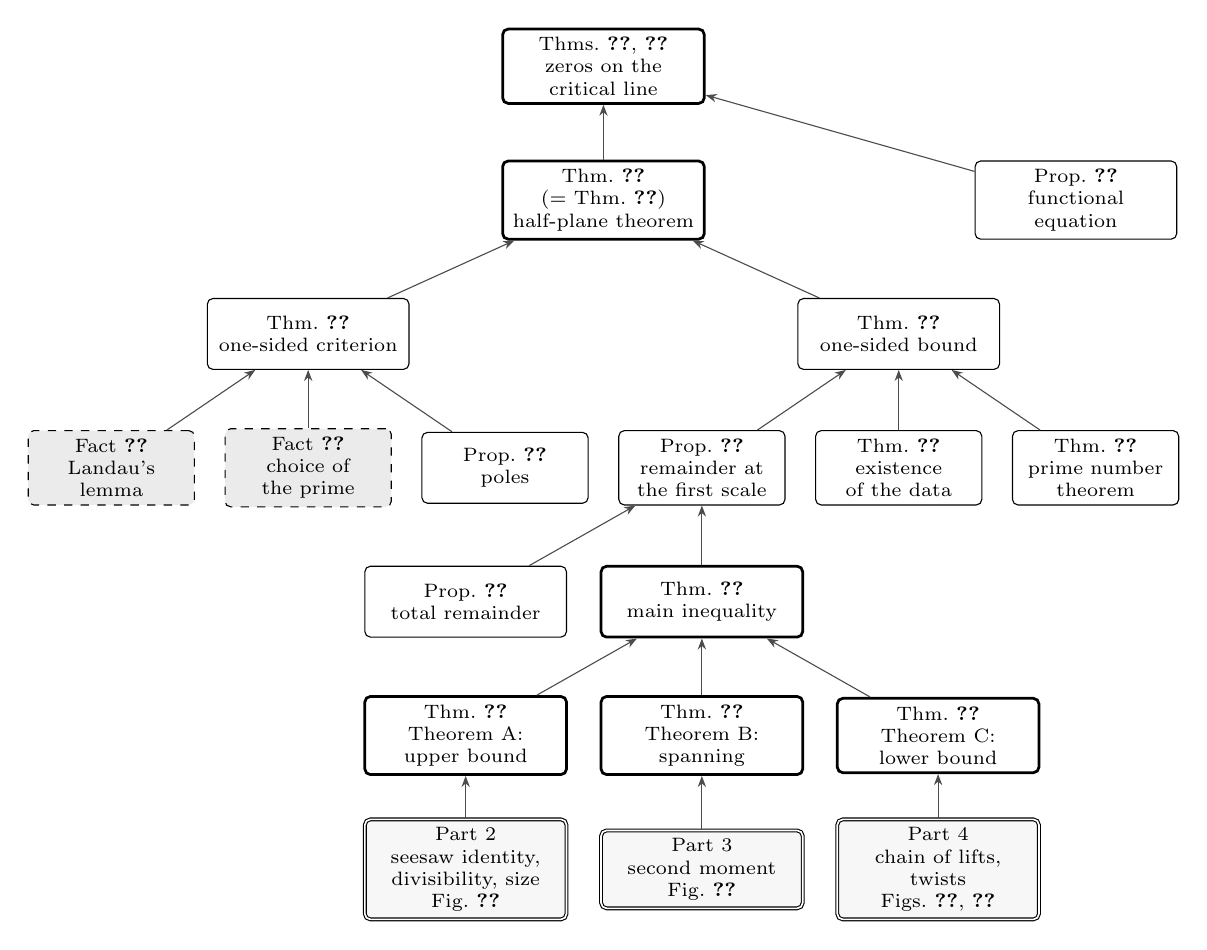
\begin{tikzpicture}[x=1cm,y=1cm]
% row 0: the statements on the critical line
\node[pfmain] (line) at (0,0) {Thms.~\ref{intro:thm:line}, \ref{intro:thm:rh}\\zeros on the critical line};
% row 1
\node[pfmain] (grh) at (0,-1.7) {Thm.~\ref{main:thm:grh}\\(=~Thm.~\ref{intro:thm:grh})\\half-plane theorem};
\node[pfnode] (fe) at (6,-1.7) {Prop.~\ref{zeros:prop:line}\\functional equation};
% row 2
\node[pfnode] (crit) at (-3.75,-3.4) {Thm.~\ref{zeros:thm:criterion}\\one-sided criterion};
\node[pfnode] (one) at (3.75,-3.4) {Thm.~\ref{main:thm:onesided}\\one-sided bound};
% row 3
\node[pffact, text width=1.9cm] (landau) at (-6.25,-5.1) {Fact~\ref{zeros:fact:landau}\\Landau's lemma};
\node[pffact, text width=1.9cm] (prime) at (-3.75,-5.1) {Fact~\ref{zeros:fact:prime}\\choice of the prime};
\node[pfnode, text width=1.9cm] (poles) at (-1.25,-5.1) {Prop.~\ref{zeros:prop:poles}\\poles};
\node[pfnode, text width=1.9cm] (atx) at (1.25,-5.1) {Prop.~\ref{main:prop:atx}\\remainder at the first scale};
\node[pfnode, text width=1.9cm] (exist) at (3.75,-5.1) {Thm.~\ref{setup:thm:existence}\\existence of the data};
\node[pfnode, text width=1.9cm] (pnt) at (6.25,-5.1) {Thm.~\ref{zeros:thm:pnt}\\prime number theorem};
% row 4
\node[pfnode] (rem) at (-1.75,-6.8) {Prop.~\ref{setup:prop:rem}\\total remainder};
\node[pfmain] (star) at (1.25,-6.8) {Thm.~\ref{main:thm:star}\\main inequality};
% row 5
\node[pfmain] (A) at (-1.75,-8.5) {Thm.~\ref{main:thm:A}\\Theorem A: upper bound};
\node[pfmain] (B) at (1.25,-8.5) {Thm.~\ref{main:thm:B}\\Theorem B: spanning};
\node[pfmain] (C) at (4.25,-8.5) {Thm.~\ref{main:thm:C}\\Theorem C: lower bound};
% row 6: the parts
\node[pfpart] (P2) at (-1.75,-10.2) {Part~2\\seesaw identity,\\divisibility, size\\Fig.~\ref{fig:part2}};
\node[pfpart] (P3) at (1.25,-10.2) {Part~3\\second moment\\Fig.~\ref{fig:part3}};
\node[pfpart] (P4) at (4.25,-10.2) {Part~4\\chain of lifts,\\twists\\Figs.~\ref{fig:part4a}, \ref{fig:part4b}};
% arrows: premise -- conclusion
\draw[pfedge] (grh) -- (line);
\draw[pfedge] (fe) -- (line);
\draw[pfedge] (crit) -- (grh);
\draw[pfedge] (one) -- (grh);
\draw[pfedge] (landau) -- (crit);
\draw[pfedge] (prime) -- (crit);
\draw[pfedge] (poles) -- (crit);
\draw[pfedge] (atx) -- (one);
\draw[pfedge] (exist) -- (one);
\draw[pfedge] (pnt) -- (one);
\draw[pfedge] (rem) -- (atx);
\draw[pfedge] (star) -- (atx);
\draw[pfedge] (A) -- (star);
\draw[pfedge] (B) -- (star);
\draw[pfedge] (C) -- (star);
\draw[pfedge] (P2) -- (A);
\draw[pfedge] (P3) -- (B);
\draw[pfedge] (P4) -- (C);
\end{tikzpicture}
\caption{The top of the proof: from the theorems of the introduction down to Theorems~A, B
and~C (Sections~\ref{sec:intro}, \ref{sec:zeros}, \ref{sec:setup} and~\ref{sec:main}). Each box
is a result, with its number and a short name; a box with several numbers stands for a group of
results. An arrow from one box to another means that the proof of the second, as written in this
paper, uses the first. Bold boxes are the final theorems,
the main inequality and Theorems~A, B and~C. Dashed grey boxes are background results admitted
without proof. Double boxes stand for the parts that prove Theorems~A, B and~C; each has its own
diagram.}
\label{fig:overview}
\end{figure}


\subsubsection*{A one-sided bound suffices}
Fix a modulus $q_0$ and a prime $d$, and let $K = \Q(\sqrt{-d})$ with quadratic character
$\chiK$. Consider the weighted sum over the prime powers $n \equiv 1 \bmod q_0$ with
$\chiK(n) \ne 1$,
\[
  R_{q_0}(x) = \sum_{\substack{n \le x \\ n \equiv 1 \bmod q_0}}
     \Lambda(n)\bigl(1 - \chiK(n)\bigr)\Bigl(\frac1n - \frac1x\Bigr) - \frac{\log x}{\varphi(q_0)} - c ,
\]
with the constant $c$ for which $R_{q_0}(x) \to 0$. A theorem of Landau's type
(Section~\ref{sec:zeros}) shows that an \emph{upper} bound $R_{q_0}(x) \le x^{-1/2+\eps}$ for all
large $x$, for every $\eps > 0$ and all primes $d$ in a residue class, excludes zeros of the
$L$-functions modulo $q_0$ in $\Re s > 1/2$. The rest of the proof establishes this upper bound for one $x$ at a time.

\subsubsection*{Size against divisibility}
The upper bound is proved by the principle that drives transcendence theory and Stepanov's proof
of the Riemann hypothesis for curves: a non-zero integer cannot be both small and highly
divisible. One builds a lattice of ``integral'' objects, shows that it contains many vectors that
are small, and compares the resulting upper bound for a determinant with a lower bound that comes
from the product formula. In his remark, Alp\"oge describes the argument as a descendant of
Stepanov's, in which the high multiplicity of an auxiliary function is replaced by a chain of
theta lifts, each lift contributing one unit of multiplicity, and the length of the chain is about
$\sqrt{x}$.

The primes enter through divisibility. A theta function of an elliptic curve with complex
multiplication by $K$ has Taylor coefficients (``jets'') at the origin which, suitably
normalised, are algebraic integers; and at a prime $p$ that does \emph{not} split in $K$ a jet of
order $a$ is divisible by about $p^{a\gamma_p}$, with $\gamma_p = 1/p + 1/p^3 + \cdots$ for inert
$p$ and $\gamma_d = \frac12(1/d + 1/d^2 + \cdots)$ (Section~\ref{sec:der}). The reason is a
Frobenius congruence $\theta(\pi_p z)/\theta(z)^{q_p} \equiv 1$ modulo the prime $\pi_p$ of $K$
above $p$, of norm $q_p$: after a scaling of $z$ it makes the theta series integral up to an
exponential factor, and Legendre's formula for $a!$ does the rest. Summed over $p$ with weights
$\log p$ these exponents give half of $\sum_n \Lambda(n)(1 - \chiK(n))\cdot a/n$, a sum over
primes of the kind that occurs in $R_{q_0}$ (the factor $2$ returns because sizes are squared
norms).

\subsubsection*{The lattice}
For each large integer $x$ the proof fixes \emph{admissible data} (Section~\ref{sec:setup}): a
cyclotomic extension $E = K(\zeta)$, a CM field with $f$ infinite places; hermitian spaces over
$E$; and scales $x < x_1 < b$ with $a = xb$. \emph{Source forms} are algebraic modular forms of
weight about $a$ on a definite unitary group $\U(X_0)$. \emph{Target forms} are automorphic forms
on a unitary group $\U(Y_0)$. A Poincar\'e series construction maps source forms to target forms,
and a chain of $m \approx \sqrt{x}$ theta lifts $\Theta_\vartheta$, twisted by a character
$\vartheta$, maps target forms to algebraic modular forms on a definite group $\U(Y_m)$, where
integrality and size make sense. The target forms with the maps $\Theta_\vartheta$ are the
lattice; a family of target forms has a \emph{covolume} (its size) and an \emph{index} (its
distance from integrality).

\subsubsection*{Three theorems}
\emph{Theorem A} (the upper bound, Part~2) produces short integral vectors. A seesaw identity
rewrites the lifts of a Poincar\'e series as a combination of chains of lifts between definite
spaces, whose values are jets of CM theta functions. Their archimedean size is explicit, and their
divisibility at the non-split primes is as above. Dividing by the guaranteed power of each prime
leaves forms whose lifts have logarithmic size at most $\hmain - m\,\rem + f a\log^4 b$, where
the \emph{main amount} $\hmain$ is explicit and huge and the \emph{total remainder} $\rem$ is a combination of the remainders
$R_{q_0}$.

\emph{Theorem B} (spanning, Part~3) shows by a second-moment computation, of the type of the
Petersson formula, that few translates of the Poincar\'e map span almost all target forms.

\emph{Theorem C} (the lower bound, Part~4) bounds covolume plus twice the index from below by
$\dT\,\hmain$, $\dT$ the dimension of the target, up to small errors, for every independent family
of almost full rank. It evaluates a Gram determinant by the product formula, with a different
twist at each prime (Theorem~\ref{setup:thm:twist}). The Gram determinant $Z(\vartheta)$ of a
chain of lifts is not evaluated: exchange identities of Siegel--Weil type write $Z(1)/Z(\vartheta)$,
up to a power of the norm of the modulus, as ratios of twisted to untwisted Hecke $L$-values times
the same ratios for the $m$ single lifts; the latter are bounded through comparison operators and
lifts of characters of $\U(1)$, whose squared norms are Hecke $L$-values (Rallis inner product
formula). The main amount reappears as the height of $Z(1)/Z(\vartheta)$, with $\vartheta$ chosen
for each prime; the twists are chosen through congruences, Galois representations and Selmer
groups, which bound the denominators of the lifts.

\subsubsection*{The conclusion}
In the comparison the main amount cancels, and what remains is $m\cdot\rem \le f a\log^5 b$
(Theorem~\ref{main:thm:star}). The weights of the forms are chosen larger at a sparse set of
places of $E$ of class $-1$ modulo $q_0$; this is how the residue class modulo $q_0$ enters, and
it makes $\rem$ equal to $a\,\#\Phi_b\,R_{q_0}(x)$ up to remainders at the far larger point $x_1$,
where the classical prime number theorem suffices (Proposition~\ref{setup:prop:rem}). Dividing by
$m \approx \sqrt{x}$ gives $R_{q_0}(x) \le C x^{-1/2+6\eps}$ for data with $\log b \approx x^\eps$.

\subsection{Organisation}

Part~1 is the reduction: the analytic criterion (Section~\ref{sec:zeros}), the data and the
general lower bound for Gram determinants (Section~\ref{sec:setup}), and the derivation of the
theorem from Theorems A, B and C (Section~\ref{sec:main}); it is complete in itself, given
Theorems B and C and the results of Part~2 from which Section~\ref{sec:main} assembles Theorem~A. Parts~2, 3 and~4 prove Theorems A, B and C. Table~\ref{intro:tab:parts} lists the
sections with the folders of the Lean text that they cover. The appendices give the notation
(Appendix~\ref{sec:app-notation}), the background results admitted
(Appendix~\ref{sec:app-facts}), the steps cited without explanation
(Appendix~\ref{sec:app-open}) and the index of Lean declarations
(Appendix~\ref{sec:app-leanindex}); the references follow.

The parts are of very unequal weight. A few sections quote a percentage for a result: it is the
share, among the declarations that the final theorem \lean{riemannHypothesis} needs, of those
that are needed only through that result. The figures come from the dependency graph of the
compiled code, in which the final theorem needs $49{,}815$ declarations. By this measure almost
half ($46\%$) of the proof is needed only through Theorem~C, and most of that only through the
existence of suitable twists (Section~\ref{sec:cg-selmer}).

\begin{table}[ht]
\centering
\small
\begin{tabular}{llp{7.9cm}}
\toprule
section & subject & Lean folders under \texttt{New/} \\
\midrule
\ref{sec:zeros} & one-sided criterion & \texttt{Reduction/Zeros}, \texttt{Main} \\
\ref{sec:setup}, \ref{sec:data} & data, heights, lattices & \texttt{Reduction/Data}, \texttt{Reduction/Lattices} \\
\ref{sec:main} & main inequality & \texttt{Reduction} \\
\midrule
\ref{sec:ub-objects} & objects & \texttt{UpperBound/Kernels}, \texttt{UpperBound/Objects} \\
\ref{sec:der} & derivatives of theta functions & \texttt{Derivatives} \\
\ref{sec:ub-seesaw} & seesaw identity & \texttt{UpperBound/Seesaw} \\
\ref{sec:ub-divis} & divisibility and size & \texttt{UpperBound/Divisibility}, \texttt{UpperBound/Size} \\
\ref{sec:ub-eldiv} & elementary divisors & \texttt{UpperBound/ElementaryDivisors} \\
\midrule
\ref{sec:sp-moment} & second moment, Bessel functions & \texttt{Spanning/SecondMoment}, \texttt{Multiplicities}, \texttt{Bessel}; \texttt{Appendix/DiscreteSeries} \\
\ref{sec:sp-unfold} & unfolding & \texttt{Spanning/Unfolding} \\
\ref{sec:sp-main} & main term & \texttt{Spanning/MainTerm} \\
\ref{sec:sp-frames} & local estimates & \texttt{Spanning/Frames} \\
\ref{sec:sp-remain} & remaining terms & \texttt{Spanning/RemainingTerms} \\
\midrule
\ref{sec:det-chain} & Theorem C, chain of lifts & \texttt{Determinant/Twist}, \texttt{Norms}, \texttt{Chain}, \texttt{AuxiliaryForms} \\
\ref{sec:det-exchange} & exchange identity & \texttt{Determinant/Exchange} \\
\ref{sec:ol-values} & one lift, Hecke values & \texttt{OneLift} except \texttt{ComparisonOperator} \\
\ref{sec:ol-compare} & comparison operator & \texttt{OneLift/ComparisonOperator} \\
\ref{sec:cg-selmer} & twists, Selmer groups & \texttt{Congruences/FitTwistsExist}, \texttt{Selmer}, \texttt{GaloisRepresentations} \\
\ref{sec:cg-first} & Ribet's method & \texttt{Congruences/FirstOrder} \\
\ref{sec:cg-lifting} & local loss & \texttt{Congruences/LocalLoss}, \texttt{Lifting} \\
\bottomrule
\end{tabular}
\caption{The sections and the Lean folders they cover.}
\label{intro:tab:parts}
\end{table}

\subsection{Conventions}

\emph{Total functions.} In Lean every function is defined everywhere. Mathlib's $\zeta$ has a
value at $s = 1$, its $\Gamma$ has the value $0$ at the poles, division by zero gives $0$. Formal
statements therefore carry side conditions such as $s \ne 1$; we keep them when they matter and
otherwise write as usual.

\emph{Places.} $\Aut(\C)$ is the group of all field automorphisms of $\C$. A pair $\iota$ of a
prime $\ell$ and a field isomorphism $\C \isom \Qlbar$ is written $\iota \mid \ell$. A complex
number is integral at $\iota$ if its image has absolute value at most $1$; a quantity is bounded
``at every conjugate'' if the bound holds after applying every $\sigma \in \Aut(\C)$.

\emph{Letters.} The symbols listed in Appendix~\ref{sec:app-notation} have one meaning in the
whole paper; among them are the letters of the data of Section~\ref{sec:setup}. There are two
standing exceptions: $s$ is also a complex variable (Section~\ref{sec:zeros}) and an element of
$\Gbar$ (as in $s\nPoin$), and a bound variable may reuse a letter. Sections introduce further
symbols for their own objects and say what they mean; where a section gives a listed letter a
local meaning, it says so at that place. A twist is $\vartheta$. Constants are explicit in the
Lean text and are not optimised; we keep them.

\emph{Sizes.} Inequalities between the sizes of the data are used constantly. They compare
quantities through bounds for their logarithms, which reduces them to linear inequalities between
$\log x$, $\log x_1$, $\log b$, $\log\log b$, $\log\log x_1$ and a constant; they are proved by one
uniform mechanism (\lean{New.Data.le_of_hasLogBound}), and are quoted without proof.

\part{The reduction}
\section{From a one-sided bound to the zeros}\label{sec:zeros}

This section is classical analytic number theory. It reduces the theorem to an upper bound for
one weighted sum over primes. The Lean files are \leanfile{New/Reduction/Zeros/PrimeError},
\leanfile{New/Reduction/Zeros/Criterion}, \leanfile{New/Reduction/Zeros/PrimeNumberTheorem} and
\leanfile{New/Main}.

\subsection{The weighted prime sum}

Throughout, $d$ is a prime and $\chiK = (\cdot/d)$ is the Legendre symbol modulo $d$. When
$d \equiv 3 \bmod 4$ it is the quadratic character of the field $K = \Q(\sqrt{-d})$: for a prime
$p \ne d$ we have $\chiK(p) = 1$ if $p$ splits in $K$ and $\chiK(p) = -1$ if $p$ is inert. Let
$\Lambda$ be the von Mangoldt function and let $q \ge 1$.

\begin{definition}[\lean{New.lambdaKResidueClass}, \lean{New.logDerivMean},
\lean{New.primeRemainder}]\label{zeros:def:remainder}
For $n \ge 1$ put
\[
  \lambda_q(n) =
  \begin{cases}
    \Lambda(n)\,\bigl(1 - \chiK(n)\bigr) & \text{if } n \equiv 1 \bmod q, \\
    0 & \text{otherwise,}
  \end{cases}
  \qquad \LambdaK = \lambda_1 .
\]
For a Dirichlet character $\psi$ let $L^*(s,\psi)$ be the entire function that equals
$L(s,\psi)$ if $\psi$ is not principal and $(s-1)L(s,\psi)$ if $\psi$ is principal
(\lean{New.entireL}). Write $\psi\chiK$ for the product character modulo $qd$
(\lean{New.quadTwist}). Put
\[
  G_q(s) = \frac{1}{\varphi(q)} \Bigl( \sum_{\psi \bmod q}
     \Bigl( \frac{L^{*\prime}}{L^*}(s,\psi\chiK) - \frac{L^{*\prime}}{L^*}(s,\psi) \Bigr) - 1 \Bigr),
  \qquad c_q = \Re G_q(1),
\]
and, for real $x > 0$,
\begin{equation}\label{zeros:eq:R}
  R_q(x) = \sum_{n \le x} \lambda_q(n) \Bigl( \frac1n - \frac1x \Bigr)
           - \frac{\log x}{\varphi(q)} - c_q .
\end{equation}
\end{definition}

The weight $\lambda_q$ is non-negative and at most $2\Lambda$. For $d \equiv 3 \bmod 4$ it is
supported on the powers of primes that do not split in $K$. The function $R_q$ depends on $d$; we write $R_{d,q}$ when the
prime matters. For odd $d$ prime to $q$ the constant $c_q$ is the one for which $R_q(x) \to 0$
(Theorem~\ref{zeros:thm:pnt}). The smooth weight $1/n - 1/x$ is what the later sections produce;
it also makes $R_q$ vary slowly:

\begin{lemma}[\lean{New.abs_primeRemainder_sub_le}]\label{zeros:lem:slow}
For $1 \le y \le z$ we have $\abs{R_q(z) - R_q(y)} \le 13\,(z-y)/y$.
\end{lemma}

\begin{proof}
Let $\mathcal{E}(t) = \sum_{n \le t} \lambda_q(n) - t/\varphi(q)$. Partial summation gives
$R_q(y) = \int_1^y \mathcal{E}(t)\,t^{-2}\,dt - c_q$ for $y \ge 1$
(\lean{New.primeRemainder_eq_integral_countError_sub}), and Chebyshev's bound
$\sum_{n \le t} \Lambda(n) \le 6t$ gives $\abs{\mathcal{E}(t)} \le 13t$.
\end{proof}

\subsection{The Dirichlet series and the Laplace transform}

\begin{lemma}[\lean{New.LSeries_lambdaKResidueClass_eq_add_logDerivMean}]\label{zeros:lem:series}
Let $d$ be odd and prime to $q$. For $\Re s > 1$,
\[
  \sum_{n \ge 1} \lambda_q(n)\, n^{-s} = \frac{s}{\varphi(q)\,(s-1)} + G_q(s).
\]
\end{lemma}

\begin{proof}
By orthogonality of characters, the indicator of $n \equiv 1 \bmod q$ is
$\varphi(q)^{-1} \sum_\psi \psi(n)$. Since $-L'/L(s,\chi) = \sum \Lambda(n)\chi(n) n^{-s}$, the
left side is $\varphi(q)^{-1} \sum_\psi \bigl( L'/L(s,\psi\chiK) - L'/L(s,\psi) \bigr)$. No
$\psi\chiK$ is principal, as $d$ is odd and prime to $q$. For the principal
character $\psi_0$ modulo $q$ we have
$L^{*\prime}/L^*(s,\psi_0) = L'/L(s,\psi_0) + 1/(s-1)$. Hence the left side equals
$G_q(s) + \varphi(q)^{-1}\bigl(1 + 1/(s-1)\bigr)$.
\end{proof}

\begin{lemma}[\lean{New.integral_primeRemainder}]\label{zeros:lem:laplace}
Let $d$ be odd and prime to $q$. For $\Re s > 2$,
\[
  \int_0^\infty R_q(e^v)\, e^{(1-s)v}\, dv = \frac{G_q(s)/s - c_q}{s-1}.
\]
\end{lemma}

\begin{proof}
For $r \in \{0,1\}$ let $S_r(y) = y^{-r} \sum_{n \le y} \lambda_q(n)\, n^{r-1}$, so that the sum in
\eqref{zeros:eq:R} is $S_0(x) - S_1(x)$. Partial summation and the substitution $t = e^v$ give
$\int_0^\infty S_r(e^v) e^{(1-s)v}\,dv = D(s)/(s+r-1)$ with $D(s) = \sum \lambda_q(n) n^{-s}$
(\lean{New.LSeries_lambdaKResidueClass}). So the transform of $S_0 - S_1$ is $D(s)/(s(s-1))$. The
transforms of $v$ and of $1$ are $(s-1)^{-2}$ and $(s-1)^{-1}$. Insert
Lemma~\ref{zeros:lem:series}: the term $s/(\varphi(q)(s-1))$ of $D$ cancels the transform of
$v/\varphi(q)$, and $G_q(s)/(s(s-1)) - c_q/(s-1)$ remains.
\end{proof}

\begin{proposition}[Poles; \lean{New.isPolar_primeRemainder}]\label{zeros:prop:poles}
Let $d \equiv 7 \bmod 8$ be a prime that does not divide $q$. Then $v \mapsto R_q(e^v)$ is
measurable, $\abs{R_q(e^v)} \le C e^v$ for $v \ge 0$ with a constant $C$, and the function
$F(s) = \int_0^\infty R_q(e^v) e^{(1-s)v}\,dv$ continues from $\Re s > 2$ to a meromorphic function
on $\C$. In $\Re s > 0$ its poles are at most simple. It has no pole at $s = 1$, and at
$\rho \ne 1$ with $\Re \rho > 0$ its residue is
\begin{equation}\label{zeros:eq:residue}
  r(\rho) = \frac{1}{\varphi(q)\,\rho\,(1-\rho)} \sum_{\psi \bmod q}
     \Bigl( \ord_{\rho} L^*(\cdot,\psi) - \ord_{\rho} L^*(\cdot,\psi\chiK) \Bigr).
\end{equation}
\end{proposition}

\begin{proof}
Of the condition $d \equiv 7 \bmod 8$ only the oddness of $d$ is used (in
Lemma~\ref{zeros:lem:laplace}). One may take $C = \abs{c_q} + 5$, as $0 \le \lambda_q(n) \le 2n$
(\lean{New.abs_primeRemainder_exp_le}). By Lemma~\ref{zeros:lem:laplace},
$F(s) = (G_q(s)/s - c_q)/(s-1)$, and the right side is
meromorphic on $\C$. A logarithmic derivative has simple poles, with residue the order of
vanishing. So $G_q$ has at most a simple pole at $\rho$, of residue
$\varphi(q)^{-1} \sum_\psi (\ord_\rho L^*(\cdot,\psi\chiK) - \ord_\rho L^*(\cdot,\psi))$
(\lean{New.tendsto_sub_mul_logDerivMean}); dividing by $\rho(\rho - 1)$ gives
\eqref{zeros:eq:residue}. No $L^*$ vanishes on $\Re s \ge 1$, so $G_q$ is analytic there, and
$G_q(x)/x - c_q = (x-1)F(x)$, real for $x > 2$, is real for $x \ge 1$ by the identity theorem
(\lean{New.ofReal_re_logDerivMean_one}). So $G_q(1) = c_q$: no pole at $1$.
\end{proof}

With the weight $1 - \chiK(n)$ the twists enter \eqref{zeros:eq:residue} with a minus sign; the
next two facts deal with this.

\subsection{Two inputs: Landau's lemma and the choice of the prime}

\begin{fact}[Landau's lemma; \lean{New.IsPolar.landau}]\label{zeros:fact:landau}
Let $E \colon \R \to \R$ be measurable with $\abs{E(v)} \le C e^v$ for $v \ge 0$, and suppose that
$\int_0^\infty E(v) e^{(1-s)v}\,dv$ continues from $\Re s > 2$ to a meromorphic function whose
poles in $\Re s > 0$ are at most simple, with residue $r(\rho)$ at $\rho$. Let $\beta > 0$. If
$E(v) \le e^{(\beta-1)v}$ for all large $v$, and $\Re r(x) \ge 0$ for every real $x > \beta$, then
$r(\rho) = 0$ for every $\rho$ with $\Re \rho > \beta$.
\end{fact}

This is a form of Landau's theorem that the Laplace transform of a non-negative function is
singular at the real point of its abscissa of convergence (Montgomery and Vaughan,
Multiplicative number theory I, 2007, Lemma~15.1). One applies it to
$K e^{(\beta-1)v} - E(v)$, non-negative on $v > 0$ for a suitable constant $K$, whose transform is $K/(s-\beta)$ minus that of $E$ (\lean{New.exists_measure_laplace_eq}), with
residue $-r(\rho)$ at $\rho$ if $\Re\rho > \beta$. Were its abscissa of convergence $\sigma_0 >
\beta$, then $-r(\sigma_0) \ge 0$, as the transform is non-negative on $(\sigma_0,\infty)$; so
$r(\sigma_0) = 0$ by hypothesis, and the transform would continue analytically to $\sigma_0$,
against Landau's theorem. So it is analytic in $\Re s > \beta$, and all residues there vanish.

\begin{fact}[Choice of the prime; \lean{New.exists_entireL_quadTwist_ne_zero}]\label{zeros:fact:prime}
Let $N \ge 1$, $\beta > 1/2$ and $H \in \R$. Let $a$ be an invertible residue class modulo $N$ such
that every prime $d \equiv a \bmod N$ satisfies $d \equiv 7 \bmod 8$ and $d \nmid N$. Then there
is a prime $d \equiv a \bmod N$ such that $L(s, \xi\chiK) \ne 0$ for every character $\xi$ modulo
$N$ and every $s$ with $\Re s \ge \beta$ and $\abs{\Im s} \le H$; here $\chiK = (\cdot/d)$.
\end{fact}

This rests on a zero-density estimate for quadratic twists: for $\delta > 0$, the number of primes
$d \le X$ of the class for which some twist has a zero with $\Re s \ge 1/2 + 9\delta$,
$\abs{\Im s} \le H$ is $O(X^{1-\delta/2})$ (\lean{New.zero_density_quadTwist}), while the sum of
$\log p/p$ over the primes $p$ of the class diverges (Dirichlet). The sources
are Jutila, \emph{On mean values of Dirichlet polynomials with real characters}, 1975, and
Heath-Brown, \emph{A mean value estimate for real character sums}, 1995. The Lean file
\leanfile{Lib/Analytic/QuadraticTwist} proves a weak form: a zero of a twist in the box makes a
tail integral of its theta series large (three-lines theorem), and their sum over
$d$ is small (mean square of Jacobi symbol sums, P\'olya--Vinogradov).

\subsection{The criterion}

\begin{theorem}[One-sided criterion; \lean{New.LFunction_ne_zero_of_primeRemainder_le}]
\label{zeros:thm:criterion}
Let $q_0$ be a positive multiple of $8$, let $d_0 \equiv 7 \bmod 8$ be prime to $q_0$, and let
$\beta > 1/2$. Suppose that for every prime $d \equiv d_0 \bmod q_0$ we have
\[
  R_{d,q_0}(x) \le x^{\beta - 1} \qquad \text{for all large } x .
\]
Then $L(\rho,\psi) \ne 0$ for every Dirichlet character $\psi$ modulo $q_0$ and every
$\rho \ne 1$ with $\Re \rho > \beta$.
\end{theorem}

\begin{proof}
Every prime $d \equiv d_0 \bmod q_0$ is $\equiv 7 \bmod 8$, since $8 \mid q_0$, and is prime to
$q_0$. Apply Fact~\ref{zeros:fact:prime} with $N = q_0$ and $H = \abs{\Im \rho}$: there is such a
prime $d$ for which no $L(s,\psi\chiK)$, $\psi$ modulo $q_0$, vanishes in the box
$\Re s \ge \beta$, $\abs{\Im s} \le \abs{\Im\rho}$. Fix this $d$ and let $r$ be the residue
function of Proposition~\ref{zeros:prop:poles} for $E(v) = R_{d,q_0}(e^v)$. In the box the twisted
terms of \eqref{zeros:eq:residue} vanish, so $r(s) = n(s)/(\varphi(q_0)\,s\,(1-s))$ with
$n(s) = \sum_\psi \ord_s L^*(\cdot,\psi) \ge 0$, over $\psi$ modulo $q_0$. For real $x$ with $\beta < x < 1$ we have $x(1-x) > 0$, so $r(x) \ge 0$. For real $x \ge 1$ no
$L^*(\cdot,\psi)$ vanishes at $x$, so $n(x) = 0$ and there is no pole. The hypothesis gives
$E(v) \le e^{(\beta-1)v}$ for large $v$. By Landau's lemma (Fact~\ref{zeros:fact:landau}),
$r(\rho) = 0$. As $\rho \ne 0, 1$, this means $n(\rho) = 0$: no $L^*(\cdot,\psi)$ vanishes at
$\rho$, and $L(\rho,\psi) = L^*(\rho,\psi)$ or $L^*(\rho,\psi)/(\rho - 1)$.
\end{proof}

\begin{remark}
A one-sided bound suffices because of the sign of the residues on the real axis. All primes $d$
of the class are needed because $d$ is chosen after $\rho$, so that the zeros of the twists stay
out of the way; nothing is assumed about real zeros.
\end{remark}

\subsection{The prime number theorem for the remainder}

The proof of the one-sided bound also uses the remainder at a much larger point, where this applies:

\begin{theorem}[\lean{New.eventually_abs_primeRemainder_le}, \lean{New.tendsto_primeRemainder}]
\label{zeros:thm:pnt}
Let $d$ be an odd prime and let $q \ge 1$ be prime to $d$. For every natural number $B$ we have
$\abs{R_q(y)} \le (\log y)^{-B}$ for all large $y$. In particular $R_q(y) \to 0$.
\end{theorem}

This is the prime number theorem in progressions to a fixed modulus with an error that saves
every power of the logarithm (Siegel--Walfisz; Montgomery and Vaughan, Multiplicative number theory I, 2007, Cor.~11.19). The
Lean proof uses the crude zero-free region that the $3$--$4$--$1$ inequality gives (\leanfile{Lib/Analytic/PrimeNumberTheorem/ZeroFreeRegion}): for all large $l$
the function $G_q(s)/s$ is holomorphic and at most $l^{26}$ in absolute value on
$\Re s \ge 1 - l^{-26}$, $\abs{s} \le e^l$ (\lean{New.eventually_norm_logDerivMean_div_le}). A
Tauberian argument (\leanfile{Lib/Analytic/PrimeNumberTheorem/Tauberian}), with
Lemma~\ref{zeros:lem:slow} as the Tauberian condition, is applied to the transform of
Lemma~\ref{zeros:lem:laplace}: a high Taylor coefficient at a real point far to the right is a
Gamma-weighted mean of $R_q(e^v)$ near a given $v$, and is small by Cauchy's estimate on a disc
reaching left of $\Re s = 1$.

\subsection{From the half-plane to the critical line}

\begin{proposition}[\lean{New.zeros_on_line}, \lean{New.zeta_zeros_on_line}]\label{zeros:prop:line}
Suppose that $L(s,\chi) \ne 0$ for every Dirichlet character $\chi$ and every $s$ with
$\Re s > 1/2$, except $s = 1$ when $\chi$ is principal. Then every zero of a Dirichlet
$L$-function in the strip $0 < \Re s < 1$ has real part $1/2$, and every zero $s \ne 1$ of $\zeta$
other than $-2, -4, \dots$ has real part $1/2$.
\end{proposition}

\begin{proof}
Let $L(s,\chi) = 0$ with $0 < \Re s < 1$. The gamma factor of the completed $L$-function has no
pole at $s$, so the functional equation gives $L(1-s,\chi^{-1}) = 0$
(\lean{New.gammaFactor_eq_zero_or_LFunction_one_sub_eq_zero}, \leanfile{Lib/Analytic/ZeroSymmetry}). The hypothesis applied to both zeros gives
$\Re s \le 1/2$ and $1 - \Re s \le 1/2$. For $\zeta$ (the character modulo $1$), a zero $s \notin \{1, 0, -2, -4, \dots\}$ is one of $\pi^{-s/2}\Gamma(s/2)\zeta(s)$, which is
symmetric under $s \mapsto 1 - s$; as $\zeta(0) \ne 0$, $1 - s \ne 1$ is again a zero of $\zeta$; argue as before.
\end{proof}

\section{The data, prime sums, heights and twisted lattices}\label{sec:setup}

This section fixes the objects that depend on the length $x$ of the prime sum, defines the
quantities that the main inequality compares, and proves the general lower bound for a Gram
determinant on which Theorem~C rests. The Lean files are those of
\leanfile{New/Reduction/Data}, \leanfile{New/Reduction/PrimeSums} and
\leanfile{New/Reduction/Lattices}.

\subsection{Parameters, the field and its places}

\begin{definition}[\lean{New.Parameters}]\label{setup:def:parameters}
The \emph{parameters} are a positive integer $q_0$ divisible by $18480 = 16\cdot3\cdot5\cdot7\cdot11$
and a prime $d$ with $q_0 \mid 2(d+1)$ and $q_0 \nmid d+1$; equivalently
$d \equiv q_0/2 - 1 \bmod q_0$. Put $K = \Q(\sqrt{-d})$ and let $\chiK$ be its quadratic
character.
\end{definition}

Then $d \equiv 7 \bmod 8$ (\lean{New.Parameters.instPrimeSevenModEight}), every prime $p$ dividing
$q_0$ (or $q_1$ below) has $\chiK(p) = 1$, so splits in $K$
(\lean{New.Parameters.chiK_eq_one_of_dvd}), and a prime that does not split in $K$ is at least
$13$ (\lean{New.Parameters.thirteen_le_of_chiK_ne_one}).

For an integer $s \ge 1$ let $l_0$ be the least power of $3$ above $27s$, and put
\[
  T = 3\, l_0\, 2^s, \qquad q_1 = q_0 T, \qquad q_2 = (q_0 d)^{s+6}
\]
(\lean{New.towerDeg}, \lean{New.Parameters.q₁}, \lean{New.Parameters.q₂}). Let $E = K(\zeta)$ with
$\zeta$ a primitive $q_1$-th root of unity (\lean{New.Parameters.E}). The cyclotomic polynomial of
order $q_1$ is irreducible over $K$ (\lean{New.Parameters.irreducible_cyclotomic}), so
$\Gal(E/K) \cong (\Z/q_1)^\times$; the field $E$ is a CM field, abelian over $\Q$. Each infinite
place of $E$ is complex, and a fixed embedding $E \to \C$ over $K$ composed with the elements of
$\Gal(E/K)$ gives one embedding for each place. So the set $\Phi$ of infinite places of $E$ is
identified with the group $(\Z/q_1)^\times$ (\lean{New.Parameters.placeMulEquiv}), and these
embeddings form a CM type. We write $f = \#\Phi = T\varphi(q_0)$, and for an integer $\nu$ prime to
$q_1$ and $\tau \in \Phi$ we write $\nu\tau$ for the product of $\tau$ with the place of the class
of $\nu$. A place has a \emph{class modulo $q_0$}, its image in $(\Z/q_0)^\times$; exactly $T$
places have class $1$ (\lean{New.Parameters.card_placeClass_eq_one_eq_towerDeg}). Finally
\[
  \Omega = \exp\bigl(\gamma - \Re \tfrac{L'}{L}(1,\chiK)\bigr)\cdot \frac{2\pi}{\rdE},
\]
with $\gamma$ Euler's constant and $\rdE$ the root discriminant of $E$
(\lean{New.Parameters.bigOmega}).

\subsection{Admissible data}

\begin{definition}[\lean{New.Data}]\label{setup:def:data}
\emph{Admissible data} $D$ for the parameters $(q_0, d)$ consist of the following.
\begin{enumerate}[label=(\alph*)]
\item \emph{Scales}: integers $x$, $x_1$, $b$ with
  $(\log b)^{100} \le x$, $x^{10^6} \le x_1$, $x_1^{10^6} \le b$, $(\log x_1)^6 \le \log b$ and
  $\log\log b \ge 10^{12} c_P$, where $c_P$ is a constant that depends on $q_0$ and $d$ only
  (\lean{New.Parameters.constantBound}). Put $a = x b$.
\item \emph{Ranks}: a power of two $m \in [\sqrt{x}, 2\sqrt{x}]$, the number of lifts; a power of
  three $r \in [x^5, 3x^5]$; and the exponent $s$ with $2^s = m^{22}$, which fixes $E$, $q_1$ and
  $q_2$ as above, with $s \le 32 \log x$. Further $q_1 x_1$ divides $b$. Put
  \[
    k = r + 1 - m, \qquad t = 5r, \qquad n_j = k + j(t+1), \qquad \Delta = 2r^8 .
  \]
\item \emph{Places}: the set $\Phi_a$ of \emph{$a$-places}, the $T$ places of class $1$ modulo
  $q_0$, and a set $\Phi_b$ of \emph{$b$-places}, all of class $-1$ modulo $q_0$, with
  $\#\Phi_b \ge T/\log b$, that is \emph{sparse}: for every prime $\ell \le kt$ and all
  $0 < i < j < l_0$ there are no $\sigma, \tau, \rho \in \Phi_b$ with
  $\tau/\sigma \equiv \pm\ell^i$ and $\rho/\sigma \equiv \pm\ell^j$ (independent signs) modulo the
  part of $q_1$ prime to $\ell$ (\lean{New.Parameters.IsSparse}).
\item \emph{Weights}: $\kappa(\tau) = b = a/x$ for $\tau \in \Phi_b$ and $\kappa(\tau) = a/x_1$
  for all other places; and $\kappa_j(\tau) = \kappa(\tau) + (j + \tfrac12)\Delta$, the weight of
  the $j$-th lift.
\item \emph{Primes}: distinct primes $p_0, p_1 \in [b^{10}, b^{11}]$ and a prime $N$, all
  $\equiv 1 \bmod q_2^2$, with an integer of $K$ of norm $M = p_0 p_1$ (its conjugate is written
  $\pi_M$) and an integer $\pi_N$ of $E$ with $\pi_N \overline{\pi_N} = N$. The level $N$ satisfies
  $\log N_- \le \log N \le \log N_- + \sqrt{\log b}$, where
  \[
    N_- = \bar\kappa^{\,m}\, \Bigl( \frac{M\,\rdE}{2\pi} \Bigr)^{m-1} b^{-15/2}
  \]
  and $\bar\kappa$ is the geometric mean of the weights $\kappa(\tau)$ over the $f$ places.
\end{enumerate}
\end{definition}

Table~\ref{setup:tab:sizes} lists the sizes. All of them follow from the definition
(\leanfile{New/Reduction/Data/Sizes}, \leanfile{New/Reduction/Data/Magnitudes},
\leanfile{New/Reduction/Data/LevelAndTwists}; for $\rdE$, \lean{New.Data.rootDisc_mem_Icc}). In the Lean text
each quantity carries an upper and a lower bound for its logarithm, and an inequality between two
quantities is proved by comparing these bounds, which is a linear problem in $\log x$, $\log x_1$,
$\log b$, $\log\log b$, $\log\log x_1$ and $c_P$ (\lean{New.Data.le_of_hasLogBound}). We use such
inequalities freely and cite them by this name.

\begin{table}[ht]
\centering
\begin{tabular}{lll}
\toprule
quantity & role & size \\
\midrule
$\log x_1$, $\log b$ & scales & $(\log x_1)^6 \le \log b$, $(\log b)^{100} \le x$ \\
$m$ & number of lifts & $[\sqrt{x}, 2\sqrt{x}]$ \\
$r$, $k$, $t$ & ranks & $r \in [x^5, 3x^5]$, $r/2 \le k \le r$, $t = 5r$ \\
$s$, $l_0$ & tower & $s \le 32\log x$, $27s < l_0 \le 81s$ \\
$T$, $f$, $q_1$ & places & $x^{11} \le m^{22} = 2^s \le T \le f \le q_1 \le x^{12}$ \\
$\rdE$, $1/\Omega$ & field & $[x^{10}, x^{12}]$, $[1, x^{13}]$ \\
$\Delta$ & gap of weights & $2r^8$ \\
$a$, $\kappa(\tau)$ & orders & $a = xb$, $\ a/x_1 \le \kappa(\tau) \le b$ \\
$M = p_0p_1$ & principal level & $[b^{20}, b^{22}]$ \\
$N$ & level & $\log N \in [m\log b, 30\, m\log b]$ \\
$f a \log^3 b$ & unit of the errors & \lean{New.Data.errorUnit} \\
\bottomrule
\end{tabular}
\caption{Sizes of admissible data. In increasing order: $\log b$, $x$, $x_1$, $b$, $M$, $N$.}
\label{setup:tab:sizes}
\end{table}

\begin{theorem}[Existence of the data; \lean{New.eventually_exists_data}]\label{setup:thm:existence}
Let $0 < \eps < 1/100$. For every large integer $x$ there are admissible data with first scale
$x$, with $x_1 = \floor{\exp(x^{\eps/6})}$ and with $x^\eps \le \log b \le x^\eps + 1$.
\end{theorem}

The proof is a construction (\leanfile{New/Reduction/Data/Existence}). The $b$-places are the
places $-g^e$, $g = 1 + 3l_0q_0$, with $e$ in a Behrend-type set without solutions of several
linear equations at once (\lean{New.exists_three_term_free}; Behrend, 1946; Shapira, 2006): a
forbidden triple of places would give a solution. The primes come from the prime number theorem in progressions, with the logarithm of
the prime in a prescribed window (\leanfile{Lib/Analytic/Primes}); the integer of norm $M$ from a
pigeonhole in the class group of $K$; $\pi_N$ from $N \equiv 1 \bmod 4$, a sum of two squares.

\subsection{Prime sums}

\begin{definition}[\lean{New.Data.primeSum}, \lean{New.Data.jetSize},
\lean{New.Data.directionAmount}, \lean{New.Data.mainAmount}, \lean{New.Data.mainPrimeSum},
\lean{New.Data.totalRemainder}]\label{setup:def:primesums}
For real $y \ge 0$, a place $\tau$ and an integer $j \ge 0$ put
\[
  \sfin(y,\tau) = \sum_{1 \le \nu \le a} \LambdaK(\nu)\,
     \Bigl( \frac{y}{\nu} - \kappa(-\nu\tau) \Bigr)_{\!+},
  \qquad
  \sinf(j) = \log j! + j \log\frac{M}{\Omega},
\]
where $u_+ = \max(u,0)$. (If $\nu$ is not prime to $q_1$, $-\nu\tau$ is read as $\tau$; then
$\LambdaK(\nu) = 0$ anyway, as $\Lambda$ lives on prime powers and $\chiK(p) = 1$ for $p \mid q_1$.) The \emph{direction amount}, the \emph{main amount}, the \emph{expected value} and
the \emph{total remainder} are
\begin{align*}
  \hdir &= \sum_{\tau \in \Phi} \bigl( \sinf(\kappa(\tau)) - \sfin(\kappa(\tau),\tau) \bigr),
  & \hmain &= m\,k\,\hdir, \\
  \smain &= a\,\Bigl( \log a - \frac1f \sum_{\tau\in\Phi} \log\kappa(\tau) + c_1 \Bigr),
  & \rem &= \sum_{\tau \in \Phi_a} \bigl( \sfin(a,\tau) - \smain \bigr),
\end{align*}
with $c_1 = \Re G_1(1)$ as in Definition~\ref{zeros:def:remainder}.
\end{definition}

The quantity $\sinf(j)$ is the logarithmic size charged to a derivative of order $j$ of a theta
function, and $\sfin(y,\tau)$ is the sum of $2v_p\log p$ over the primes $p$ that do not split in $K$,
with $p^{v_p}$ the predicted divisibility of such a derivative (Section~\ref{sec:der}). The main amount is
large and positive: $\hmain \ge x^4 f a$ (\lean{New.Data.le_mainAmount}). It will cancel. What
does not cancel is the total remainder, and it is a combination of the remainders of
Section~\ref{sec:zeros}:

\begin{proposition}[\lean{New.Data.totalRemainder_eq}]\label{setup:prop:rem}
\[
  \rem = a\,\Bigl( \#\Phi_b\,\bigl( R_{q_0}(x) - R_{q_0}(x_1) \bigr) + \#\Phi_a\, R_1(x_1) \Bigr).
\]
\end{proposition}

\begin{proof}
Fix $\nu \le a$ prime to $q_1$ (for other $\nu$ both sides of the next display vanish) and let
$\tau$ run over $\Phi_a$. Then $-\nu\tau$ runs once over
the places of the class of $-\nu$ modulo $q_0$. The $b$-places have class $-1$. So $-\nu\tau$ is a
$b$-place for exactly $\#\Phi_b$ values of $\tau$ if $\nu \equiv 1 \bmod q_0$, and for none
otherwise (\lean{New.Data.card_filter_mem_bPlaces}). As $\kappa = a/x$ on $\Phi_b$ and
$\kappa = a/x_1$ elsewhere,
\[
  \sum_{\tau\in\Phi_a} \LambdaK(\nu)\Bigl(\frac a\nu - \kappa(-\nu\tau)\Bigr)_{\!+}
  = \#\Phi_a\,\lambda_1(\nu)\Bigl(\frac a\nu - \frac a{x_1}\Bigr)_{\!+}
  + \#\Phi_b\,\lambda_{q_0}(\nu)\Bigl[\Bigl(\frac a\nu - \frac a{x}\Bigr)_{\!+}
       - \Bigl(\frac a\nu - \frac a{x_1}\Bigr)_{\!+}\Bigr].
\]
For $0 < z \le a$, the definition \eqref{zeros:eq:R} gives
$\sum_{\nu \le a} \lambda_q(\nu)(a/\nu - a/z)_+ = a\,(R_q(z) + \log z/\varphi(q) + c_q)$
(\lean{New.sum_lambdaKResidueClass_mul_posPart}). Summing over $\nu$,
\[
  \sum_{\tau\in\Phi_a} \sfin(a,\tau)
  = a\,\Bigl( \#\Phi_a\bigl(R_1(x_1) + \log x_1 + c_1\bigr)
     + \#\Phi_b\Bigl(R_{q_0}(x) - R_{q_0}(x_1) + \frac{\log(x/x_1)}{\varphi(q_0)}\Bigr) \Bigr);
\]
the constant $c_{q_0}$ has cancelled. On the other hand
$\sum_\tau \log\kappa(\tau) = f\log(a/x_1) - \#\Phi_b\log(x/x_1)$
(\lean{New.Data.sum_log_weight}) and $f = \#\Phi_a\,\varphi(q_0)$, so $\#\Phi_a\,\smain = a\,(\#\Phi_a(\log x_1 + c_1) + \#\Phi_b\log(x/x_1)/\varphi(q_0))$
(\lean{New.Data.card_aPlaces_mul_mainPrimeSum}). Subtract.
\end{proof}

Hence the two kinds of places: only $\nu \equiv 1 \bmod q_0$ moves an $a$-place to a $b$-place,
where the weight is larger, so the class modulo $q_0$, and with it the Dirichlet characters
modulo $q_0$, enters through the weights alone.

\subsection{Heights}

Let $\mathcal{I}$ be the set of pairs $\iota = (\ell, \iota)$ of a prime $\ell$ and a field
isomorphism $\iota \colon \C \isom \Qlbar$ (\lean{New.PrimePadicIso}); we write $\iota \mid \ell$,
and $\norm{\cdot}_\ell$ for the absolute value of $\Qlbar$ with $\norm{\ell}_\ell = \ell^{-1}$. A
complex number $z$ is \emph{integral at $\iota$} if $\norm{\iota z}_\ell \le 1$. The conjugate
isomorphism is $\bar\iota(z) = \iota(\bar z)$.

\begin{definition}[\lean{New.HeightLe}]\label{setup:def:height}
A family $y = (y_\iota)_{\iota \in \mathcal{I}}$ of complex numbers has \emph{height at most $c$}
if there are a complex number $H \ne 0$, a real number $\alpha$ and real numbers $h_\ell \ge 0$
such that
\[
  \abs{\sigma H} \le e^{\alpha} \ \text{ for all } \sigma \in \Aut(\C), \qquad
  \norm{\iota(H y_\iota)}_\ell \le \ell^{h_\ell} \ \text{ for all } \iota \mid \ell, \qquad
  \alpha + \sum_{\ell \in S} h_\ell \log \ell \le c
\]
for every finite set $S$ of primes.
\end{definition}

The multiplier $H$, and with it the bound at infinity, is the same for all $\iota$, while the
number $y_\iota$ may depend on $\iota$. This is what later lets each prime use its own twist.
Heights add under pointwise products and powers (\lean{New.HeightLe.mul}, \lean{New.HeightLe.pow})
and are monotone (\lean{New.HeightLe.mono}); they may be negative.

\begin{lemma}[Product formula; \lean{New.HeightLe.neg_le_of_norm_map_le}]\label{setup:lem:product}
Let $z \ne 0$ be a complex number. If the constant family $z$ has height at most $c$, and
$\abs{\sigma z} \le e^{c'}$ for all $\sigma \in \Aut(\C)$, then $c + c' \ge 0$.
\end{lemma}

\begin{proof}
Take $H$, $\alpha$, $h_\ell$ as in the definition and put $w = Hz \ne 0$. All conjugates
$\sigma w$ are bounded by $e^{\alpha + c'}$, and $\norm{\iota w}_2 \le 2^{h_2}$ for all $\iota \mid 2$;
the latter makes $w$ algebraic (\lean{New.isAlgebraic_of_norm_complexToCp_le}), of some degree
$n$. Its norm
$\Nm(w) \in \Q^\times$ has $\abs{\Nm(w)} \le e^{n(\alpha + c')}$ and
$\norm{\Nm(w)}_\ell \le \ell^{n h_\ell}$ for each prime $\ell$
(\lean{New.HeightLe.norm_algebraMap_norm_gen_le}). By the product formula for $\Q$,
$0 = \log\abs{\Nm(w)} + \sum_\ell \log\norm{\Nm(w)}_\ell \le n(\alpha + c') + n\sum_\ell h_\ell\log\ell
\le n(c + c')$, the sums being over the finitely many $\ell$ with $\norm{\Nm(w)}_\ell \ne 1$.
\end{proof}

\subsection{Twisted lattices}

\begin{definition}[\lean{New.TwistedLattice}]\label{setup:def:lattice}
Let $V$ be a complex vector space and $\mathcal{T}$ a set with a distinguished element $1$, whose
elements are called \emph{twists}; inner products are linear in the second variable. A \emph{twisted lattice} on $V$ consists of
\begin{itemize}
\item for each twist $\xi$ a complex inner product space $U_\xi$ and a linear map
  $\Theta_\xi \colon V \to U_\xi$;
\item for each prime $\ell$ a set of twists \emph{allowed at $\ell$};
\item for each $\xi$ and each $\iota \mid \ell$ a module $U_\xi(\iota) \subset U_\xi$ over the
  ring $\cO_\iota$ of complex numbers integral at $\iota$, the vectors \emph{integral at $\iota$},
  such that $\pair{\varphi, \varphi'}$ is integral at $\iota$ whenever $\xi$ is allowed at $\ell$,
  $\varphi \in U_\xi(\bar\iota)$ and $\varphi' \in U_\xi(\iota)$;
\item finitely many linear forms on $U_1$, the \emph{coordinates}, in which the inner product has a
  rational matrix that is positive definite on the whole coordinate space.
\end{itemize}
A vector $v \in V$ is \emph{integral at $\iota \mid \ell$} if $\Theta_\xi v \in U_\xi(\iota)$ for
every twist $\xi$ allowed at $\ell$ (\lean{New.TwistedLattice.integralVectors}).
\end{definition}

For $\sigma \in \Aut(\C)$ and $v \in V$ let $\sigma\Theta_1 v$ be the coordinate vector of
$\Theta_1 v$ with $\sigma$ applied to each coordinate, and pair such vectors by the rational
matrix. Write $\norm{\Theta_1 v}_\sigma^2$ for the product of $\sigma\Theta_1 v$ with itself
(\lean{New.TwistedLattice.normSqAt}).

\begin{definition}[\lean{New.TwistedLattice.IndexLe}, \lean{New.TwistedLattice.CovolumeLe},
\lean{New.TwistedLattice.volume}]\label{setup:def:index}
Let $y = (y_1, \dots, y_n)$ be a family in $V$.
\begin{itemize}
\item $y$ has \emph{index at most $\delta$} if there are $\delta_\ell \ge 0$ with
  $\sum_{\ell \in S}\delta_\ell\log\ell \le \delta$ for all finite sets $S$ of primes, such that
  for every $\iota \mid \ell$ some $n \times n$ matrix $u$ over $\cO_\iota$ with
  $\norm{\iota(\det u)}_\ell \ge \ell^{-\delta_\ell}$ has all combinations $\sum_k u_{ik} y_k$
  integral at $\iota$. The matrix does not depend on the twist.
\item $y$ has \emph{covolume at most $c$} if
  $\abs{\det(\pair{\sigma\Theta_1 y_i, \sigma\Theta_1 y_k})_{i,k}} \le e^{c}$ for every
  $\sigma \in \Aut(\C)$.
\end{itemize}
If $V$ is a finite-dimensional inner product space, put $Z(\xi) = \det(\Theta_\xi^*\Theta_\xi)$,
the Gram determinant of the images under $\Theta_\xi$ of an orthonormal basis of $V$.
\end{definition}

The index measures how far the family is from integral, at the same price for all twists; the
covolume measures its size, for the trivial twist only. By Hadamard's inequality,
if $\norm{\Theta_1 y_i}_\sigma^2 \le e^h$ for all $i$ and $\sigma$, then $y$ has covolume at most
$nh$ (\lean{New.TwistedLattice.covolumeLe_of_normSqAt_le}).

\begin{theorem}[A twist for each prime; \lean{New.TwistedLattice.covolume_add_index_nonneg}]
\label{setup:thm:twist}
Let $V$ be a finite-dimensional inner product space with a twisted lattice all of whose maps
$\Theta_\xi$ are injective. Let $y_1, \dots, y_n, z_1, \dots, z_{n'}$ be a basis of $V$, and for
each $\iota \mid \ell$ let $\xi_\iota$ be a twist allowed at $\ell$. Suppose that
\begin{enumerate}[label=(\roman*)]
\item $y$ has covolume at most $c$ and index at most $\delta$;
\item for each twist $\xi$ there is a number $\gamma(\xi) \ne 0$ such that
  $\gamma(\xi)\Theta_\xi z_i$ is integral at every $\iota \mid \ell$ for which $\xi$ is allowed at
  $\ell$;
\item $\norm{\Theta_1 z_i}_\sigma^2 \le e^{b_{\mathrm{short}}}$ for all $i$ and all
  $\sigma \in \Aut(\C)$;
\item the families $\iota \mapsto \abs{\gamma(\xi_\iota)}^{-2}$ and
  $\iota \mapsto Z(1)/Z(\xi_\iota)$ have height at most $b_{\mathrm{denom}}$ and
  $b_{\mathrm{vol}}$.
\end{enumerate}
Then
\[
  c + 2\delta + n'\,(b_{\mathrm{short}} + b_{\mathrm{denom}}) + b_{\mathrm{vol}} \ge 0 .
\]
\end{theorem}

\begin{proof}
Let $w = (y, z)$ and let $\mathrm{Gram}(\xi)$ be the determinant of the matrix
$(\pair{\Theta_\xi w_i, \Theta_\xi w_k})$. If $B$ is the matrix of $w$ in an orthonormal basis of
$V$, then $\mathrm{Gram}(\xi) = Z(\xi)\,\abs{\det B}^2$. So for every $\iota$
\begin{equation}\label{setup:eq:factor}
  \mathrm{Gram}(1) = \Bigl[ \abs{\gamma(\xi_\iota)}^{2n'}\, \mathrm{Gram}(\xi_\iota) \Bigr]
     \cdot \Bigl[ \abs{\gamma(\xi_\iota)}^{-2} \Bigr]^{n'} \cdot \frac{Z(1)}{Z(\xi_\iota)} .
\end{equation}
The left side does not depend on $\iota$, and it is non-zero because $\Theta_1$ is injective.

\emph{The first factor has height at most $2\delta$}
(\lean{New.TwistedLattice.heightLe_pow_mul_det_gram}). Fix $\iota \mid \ell$, write
$\xi = \xi_\iota$, and let $u$ and $u'$ be the matrices of the definition of the index at $\iota$
and at $\bar\iota$. Enlarge them by the scalar block $\gamma(\xi)$ on the $z_i$. The resulting
matrices carry the vectors $\Theta_\xi w_i$ into $U_\xi(\iota)$ and into $U_\xi(\bar\iota)$. As
$\xi$ is allowed at $\ell$, all inner products between the two transformed families are integral
at $\iota$, hence so is the determinant
$\overline{\det u'}\cdot\abs{\gamma(\xi)}^{2n'}\,\mathrm{Gram}(\xi)\cdot\det u$. Since
$\norm{\iota(\det u)}_\ell$ and $\norm{\bar\iota(\det u')}_\ell$ are at least $\ell^{-\delta_\ell}$, we get
$\norm{\iota(\abs{\gamma(\xi)}^{2n'}\mathrm{Gram}(\xi))}_\ell \le \ell^{2\delta_\ell}$; this is
height at most $2\delta$, with $H = 1$ and $\alpha = 0$.

By (iv) and the additivity of heights, \eqref{setup:eq:factor} shows that the constant family
$\mathrm{Gram}(1)$ has height at most $2\delta + n' b_{\mathrm{denom}} + b_{\mathrm{vol}}$. On the
other hand, as the matrix of the inner product is rational, $\sigma\,\mathrm{Gram}(1)$ is the
determinant of the pairings of the vectors $\sigma'\Theta_1 w_i$ with the $\sigma\Theta_1 w_k$, where
$\sigma'$ is $\sigma$ conjugated by complex conjugation; by the Cauchy--Schwarz inequality for determinants its
square is at most the product of the Gram determinants of these two families. By (i), (iii) and
the inequalities of Fischer and Hadamard, each is at most $e^{c + n' b_{\mathrm{short}}}$, so
$\abs{\sigma\,\mathrm{Gram}(1)} \le e^{c + n' b_{\mathrm{short}}}$ for all $\sigma$
(\lean{New.TwistedLattice.CovolumeLe.sumElim},
\lean{New.TwistedLattice.CovolumeLe.norm_map_det_gram_le}). The product formula,
Lemma~\ref{setup:lem:product}, gives the claim.
\end{proof}

\begin{remark}
This is the determinant method of transcendence theory, by which a non-zero algebraic number
cannot be small at all places (compare Laurent's interpolation determinants, Laurent, 1994, and Bost's slope
inequalities, Bost, 2001), with a twist $\xi_\iota$ for each $\iota$; as
$\mathrm{Gram}(\xi)/Z(\xi)$ does not depend on $\xi$, the price is the height of $Z(1)/Z(\xi_\iota)$.
\end{remark}

\subsection{The lattice of target forms}

The objects named here are defined in Section~\ref{sec:ub-objects}. The \emph{target forms}
$\mathcal{T}_D$ (\lean{New.Data.targetForms}) are a finite-dimensional space of automorphic forms
on the unitary group of a hermitian space $Y_0$ over $E$; put $\dT = \dim \mathcal{T}_D$. Twists are
defined in Definition~\ref{data:def:twist}; in short, a
\emph{twist} $\vartheta$ is an automorphic character of $\U(1)$ of weight $0$ that is tamely
ramified at a finite set $Q$ of places, its \emph{modulus}, disjoint from its conjugate and of norm
prime to $MN$ (\lean{New.Data.TameChar}, \lean{New.Data.Twist}); it is \emph{$m$-fold} if
$\vartheta, \vartheta^2, \dots, \vartheta^m$ all ramify at every place of $Q$
(\lean{New.Data.MFoldTwist}). For an $m$-fold twist, the chain of $m$ theta lifts
$\Theta_\vartheta$ maps $\mathcal{T}_D$ to a space of algebraic modular forms on the definite
unitary group of $Y_m$; such forms are functions on a finite set of classes with values in a
representation with a $\Z$-structure, whence an inner product, integrality at each $\iota$ and
conjugates under $\Aut(\C)$.

\begin{proposition}[\lean{New.Data.targetLattice}]\label{setup:prop:targetlattice}
The maps $\Theta_\vartheta$, with the forms on $Y_m$ that are integral at $\iota$ as integral
vectors, and with $\vartheta$ allowed at $\ell$ if the norm of its modulus is prime to $\ell$, are
a twisted lattice on $\mathcal{T}_D$, with twists the $m$-fold twists. In it,
$\norm{\Theta_1 y}_\sigma^2$ is the squared norm of the conjugate form
(\lean{New.Data.normSqAt_targetLattice}), $Z(\vartheta)$ is the \emph{chain determinant}
$\det(\Theta_\vartheta^*\Theta_\vartheta)$ (\lean{New.Data.volume_targetLattice}), and every
$\Theta_\vartheta$ is injective (\lean{New.Data.injective_lift_targetLattice}).
\end{proposition}

Inner products are integral because the level of the forms on $Y_m$ is so small that all classes
have trivial stabilisers (\lean{New.Data.classAut_lastResidueLevel_eq_bot}); the coordinates for
the trivial twist are the values at class representatives. Injectivity is proved in
Section~\ref{sec:det-chain}.

\section{Existence of the data, twists, and colength}\label{sec:data}

This supplement to Section~\ref{sec:setup}, in its notation, proves the facts on $E$ used
elsewhere and Theorem~\ref{setup:thm:existence}, and defines twists, the characters of the lifts
and colengths (\leanfile{New/Reduction/Data},
\leanfile{New/Reduction/Lattices/Colength}). We write $h_K$ for the class number of $K$, $\F_w$ for
the residue field of a finite place $w$ of $E$, $\Nm w = \#\F_w$; a bar is complex conjugation; the
\emph{class modulo $q \mid q_1$} of a place is its image in $(\Z/q)^\times$.

\subsection{The field}

\begin{fact}[Background, standard]\label{data:fact:ant}
In \leanfile{Lib/General/NumberTheory}: (i) A number field with primitive roots of unity of
coprime orders $n, n'$ has degree $\ge \varphi(n)\varphi(n')$
(\lean{New.totient_mul_totient_le_finrank}). For a prime $d \equiv 3 \bmod 4$,
$K \subset \Q(\zeta_d)$ (\lean{New.QuadField.embOfPrimitiveRoot}). (ii) For a prime $p$, $(p)$ is
a place of $K$ of norm $p^2$, or $(p) = \fp\fp'$, $\fp, \fp'$ of norm $p$
(\lean{New.QuadField.prime_inert_or_eq_mul}); for $d \equiv 7 \bmod 8$, the latter iff
$\chiK(p) \ne -1$ (\lean{New.QuadField.q_eq_iff_chiK_ne_neg_one}); $(y)$ has norm $y\bar y$
(\lean{New.QuadField.absNorm_span_eq_mul_star}). (iii) A CM field with integers $i$, $\beta$,
$i^2 = -1$, $\bar i = -i$, $\beta + \bar\beta = 1$, is unramified over its real subfield at finite
places (\lean{New.differentIdeal_eq_top_of_add_star_eq_one}). (iv) If $q \in \Z$, $\abs q > 1$,
$q^o \equiv 1 \bmod 2^{s+1}$, $o \ge 1$: $2^s \le (\abs q + 1)o$
(\lean{New.two_pow_le_of_pow_eq_one}).
\end{fact}

\begin{proposition}[The field $E$]\label{data:prop:field}
(a) $d \equiv 7 \bmod 8$, $d > 64$, and $d^n \not\equiv -1 \bmod q_0$ for all $n \ge 0$. Every
prime $p \mid q_1$ divides $(d+1)/4$ and splits in $K$. So $\gcd(q_1,d) = 1$, and primes that do
not split in $K$ are $\ge 13$. (b) The cyclotomic polynomial of order $q_1$ is irreducible over
$K$, so $\Gal(E/K) \cong (\Z/q_1)^\times$ by $\sigma\zeta = \zeta^\nu$, $\nu \in (\Z/q_1)^\times$;
and $E \subset \Q(\zeta_{q_1d})$. (c) For a fixed $K$-embedding $\Phi_1 \colon E \to \C$,
$\sigma \mapsto$ (place of $\Phi_1\sigma$) is a bijection $\Gal(E/K) \to \Phi$; so
$\Phi \cong (\Z/q_1)^\times$, $v \mapsto \sigma_v$, with $\sigma_1 = \id$. The CM type
$\Phi_v = \Phi_1\sigma_v$ consists of all $K$-embeddings, one at each place;
$\Phi_{vv'} = \Phi_v\sigma_{v'}$ and $\prod_v \Phi_v(y) = \Nm_{E/K}(y)$. Further
$f = T\varphi(q_0)$, and exactly $T$ places have class $1$ modulo $q_0$. (d) The roots of unity
of $E$ are the powers of $\zeta$, and $\Nm_{E/K}(\zeta) = 1$. (e) $5040 = 7! \mid q_1$, so $E$
contains a primitive $5040$-th root of unity (\lean{New.HasPrimitiveRoot5040});
$\cO_E \ni i$ with $i^2 = -1$, $\bar i = -i$ (namely $i = \pm\zeta^{q_1/4}$); and $E$ is
unramified over its maximal real subfield at all finite places (``stably unramified'').
\end{proposition}

\begin{proof}
(a) (\lean{New.Parameters.chiK_eq_one_of_dvd}, \lean{New.Parameters.d_pow_ne_neg_one}) As
$q_0 \mid 2(d+1)$, $q_0 \nmid d+1$, $d+1$ is an odd multiple of $q_0/2$, so of $8$; and
$2(d+1) \ge 18480$. Modulo $q_0$, $d^2 - 1 = \frac{d-1}2\cdot2(d+1) \equiv 0$, so the powers of
$d$ are $1$ and $d$, neither $\equiv -1$ ($q_0 \nmid 2, d+1$). The primes of $T$
are $2, 3$, which divide $q_0$; so a prime $p \mid q_1$ divides
$2(d+1) = 8\cdot\frac{d+1}4$, hence $\frac{d+1}4$ (for $p = 2$ as $8 \mid d+1$). So
$d \equiv -1 \bmod 4p$ and, as the Jacobi symbol $(\frac p\cdot)$ depends only on residues modulo
$4p$, $\chiK(p) = (\frac p{4p-1}) = (\frac{4p}{4p-1}) = 1$; $\chiK(d) = 0$ gives $d \nmid q_1$.
Primes below $13$ divide $18480$.
(b) (\lean{New.Parameters.irreducible_cyclotomic}) View $K \subset \Q(\zeta_d)$. As
$\gcd(q_1,d) = 1$, Fact~\ref{data:fact:ant}(i) gives $[\Q(\zeta_d,\zeta_{q_1}):\Q(\zeta_d)] =
\varphi(q_1)$; so the cyclotomic polynomial is irreducible over $\Q(\zeta_d) \supset K$.

(c) (\lean{New.Parameters.placeMulEquiv},
\lean{New.Parameters.card_placeClass_eq_one_eq_towerDeg}) $\Gal(E/K)$ is transitive on the
places, all above that of $K$; two $K$-embeddings with the same place are equal or conjugate,
and conjugate ones differ on $K$. As the primes of $T$
divide $q_0$, the cyclotomic polynomial of order $q_1$ is that of order $q_0$ at $X^T$, so
$f = \varphi(q_1) = T\varphi(q_0)$; and $(\Z/q_1)^\times \surj (\Z/q_0)^\times$.
(d) (\lean{New.Parameters.exists_zeta_pow_eq}) A root of unity $y \in E \subset \Q(\zeta_{q_1d})$
has order dividing $q_1d$. If $y^{q_1} \ne 1$, $y^{q_1}$ is a primitive $d$-th root of unity, and
Fact~\ref{data:fact:ant}(i) gives $2\varphi(q_1) = [E:\Q] \ge (d-1)\varphi(q_1)$, against $d > 64$.
The norm of $\zeta$ is the constant term $1$ of the cyclotomic polynomial of order $q_1 > 2$.

(e) (\lean{New.differentIdeal_eq_top}) $5040 \mid 3\cdot18480 \mid q_0T$; take $\zeta^{q_1/5040}$.
Fact~\ref{data:fact:ant}(iii) applies to $i$ and $\beta = -(\eta+\eta^2+\eta^4)$, $\eta$ of order
$7$, powers of a primitive $5040$-th root: $\beta + \bar\beta = 1$, $\beta\bar\beta = 2$
(\lean{New.HasPrimitiveRoot5040.exists_add_star_eq_one_mul_star_eq_two}).
\end{proof}

\begin{remark}[The constants]\label{data:rem:constants}
Primes $p \equiv 1 \bmod q_1d$ ($p_0, p_1, N$) split completely in $E$; no $v \in \Phi$ maps a
place above $p$ to its conjugate (\lean{New.Parameters.smul_ne_star}). The factor $16$ of $18480$
gives $d \equiv 7 \bmod 8$, used in Section~\ref{sec:der}; $3l_0$, $2^s$ serve
Proposition~\ref{data:prop:sparse}.
\end{remark}

\subsection{Existence of the data}

\begin{lemma}[Behrend-type sets; \lean{New.exists_three_term_free}]\label{data:lem:behrend}
Let $n, H, c, o \ge 1$ be integers, $(cH)^n \le o$. Some $S \subset \{0, \dots, o-1\}$ with
$\#S \ge H^n/(nH^2)$ has: if $e_1, e_2, e_3 \in S$ and integers $\alpha, \alpha' > 0$,
$\alpha + \alpha' \le c$, satisfy $(\alpha+\alpha')e_2 \equiv \alpha e_1 + \alpha' e_3 \bmod o$, then
$e_1 = e_2 = e_3$.
\end{lemma}

\begin{proof}
The sums $\sum_l v_l^2$ over $v \in \{0,\dots,H-1\}^n$ take at most $nH^2$ values, so some sphere
$\sum_l v_l^2 = C$ holds $\ge H^n/(nH^2)$ of these $v$; let $S$ be the numbers
$\sum_l v_l(cH)^l$ for them. If $e_1, e_2, e_3$ have digits $u, v, w$, then $(\alpha+\alpha')v$ and
$\alpha u + \alpha' w$ have digits below $cH$, so both sides are numbers below $(cH)^n \le o$ in
base $cH$, and $(\alpha+\alpha')v = \alpha u + \alpha' w$. Then
$\alpha\alpha'\abs{u-w}^2 = (\alpha+\alpha')(\alpha\abs u^2 + \alpha'\abs w^2)
- \abs{\alpha u+\alpha'w}^2 = 0$, so $u = w = v$.
\end{proof}

\begin{proposition}[A sparse set of $b$-places; \lean{New.Parameters.exists_large_isSparse},
\lean{New.Parameters.exists_isSparse}]\label{data:prop:sparse}
Let $n, H, B \ge 1$ with $(2l_0H)^n \le 2^s$ and $2l_0(B+1) < 2^s$. Some set of $\ge H^n/(nH^2)$
places of class $-1$ modulo $q_0$ is sparse for the primes $\ell \le B$ (as in
Definition~\ref{setup:def:data}(c), where $B = kt$). If $1 \le W \le 2^s \le W^n$,
$(2l_0)^n \le W$ and $3l_0n2^n \le W^3$, such a set $\Phi_b$ exists with $T \le \#\Phi_b\, W^6$.
\end{proposition}

\begin{proof}
Write $q_0 = 2^hu$, $u$ odd, $h \ge 4$. As $3l_0u$ is odd, $g = 1 + 3l_0q_0$ has order $2^s$
modulo $2^{s+h}$, a divisor of $q_1$ (\lean{New.Parameters.exists_orderOf_placeClass_eq}). Take
$S$ from Lemma~\ref{data:lem:behrend} with $c = 2l_0$, $o = 2^s$, and let $\Phi_b$ be the places
$-g^e$, $e \in S$, distinct and $\equiv -1 \bmod 3l_0q_0$.

Let $\sigma, \tau, \rho \in \Phi_b$, named by $-g^{e_1}, -g^{e_2}, -g^{e_3}$, have
$\tau/\sigma \equiv \pm\ell^i$, $\rho/\sigma \equiv \pm\ell^j$ modulo the part of $q_1$ prime to
$\ell$, with $\ell \le B$ prime and $0 < i < j < l_0$; squaring removes the signs. If $\ell = 2$,
then modulo $3l_0 = 3^{c'}$ we have $\tau/\sigma = g^{e_2-e_1} \equiv 1$, so $4^i \equiv 1$; but
$4 = 1+3$ has order $3^{c'-1} = l_0 > i$. If $\ell$ is odd, then modulo $2^{s+h}$,
$g^{2(e_2-e_1)} \equiv \ell^{2i}$ and $g^{2(e_3-e_1)} \equiv \ell^{2j}$ give
$g^{2j(e_2-e_1)} \equiv g^{2i(e_3-e_1)}$, that is
$(\alpha+\alpha')e_2 \equiv \alpha e_1 + \alpha'e_3 \bmod 2^s$ with $\alpha = 2(j-i)$,
$\alpha' = 2i$, $\alpha + \alpha' < 2l_0$. So $e_1 = e_2$, $\tau = \sigma$, and
$\ell^{2i} \equiv 1 \bmod 2^{s+1}$; Fact~\ref{data:fact:ant}(iv) gives
$2^s \le (\ell+1)2i < 2l_0(B+1) < 2^s$. For the count take $H$ a power of $2$ with
$H^n \le 2^s/W < (2H)^n$. Then $(2l_0H)^n \le 2^s$, $H \le W$, and
$T = 3l_02^s < \frac{H^n}{nH^2}\cdot3l_0n2^nWH^2 \le \#\Phi_bW^6$.
\end{proof}

\begin{fact}[Primes in windows; \lean{New.exists_prime_modEq_one_log_mem}]\label{data:fact:primes}
Let $u, A \ge 1$ be integers, $4 \mid u$. For all large real $W$, all $e > 1$ with
$u^e \le W^A$ and all $U \in [W, W^A]$, some prime $p \equiv 1 \bmod u^e$ has
$\log p \in [U, U + W]$. (\leanfile{Lib/Analytic/Primes}, by Newman's method; cf.\
Siegel--Walfisz, Montgomery and Vaughan, Multiplicative number theory I, 2007, Cor.~11.19.)
\end{fact}

\begin{lemma}[$p_0, p_1, \pi_M$; \lean{New.Parameters.exists_prime_pair_norm}]\label{data:lem:pair}
Let $L, W > 0$, $(2h_K+2)W \le L$, and let each window $[U, U+W]$ with $10L \le U \le 11L$
contain $\log p$ for a prime $p \equiv 1 \bmod q_2^2$. Then two distinct such primes
$p_0, p_1 \in [e^{10L}, e^{11L}]$ have $p_0p_1 = \alpha\bar\alpha$, $\alpha \in \cO_K$.
\end{lemma}

\begin{proof}
The disjoint windows at $10L + 2iW$, $0 \le i \le h_K$, give primes
$p^{(i)} \equiv 1 \bmod d$; by Fact~\ref{data:fact:ant}(ii), $(p^{(i)}) = \fp_i\fp'_i$, both of norm
$p^{(i)}$. Two classes agree, $[\fp_i] = [\fp_j]$,
$i \ne j$; then $[\fp_i\fp'_j] = [\fp_j\fp'_j] = 1$, so $\fp_i\fp'_j = (\alpha)$ and
$\alpha\bar\alpha = p^{(i)}p^{(j)}$ (\lean{New.exists_ne_isPrincipal_mul}).
\end{proof}

\begin{lemma}[$N, \pi_N$; \lean{New.Parameters.exists_prime_log_mem_Icc_mul_star_eq}]
\label{data:lem:level}
(a) A prime $N \equiv 1 \bmod 4$ is $\pi\bar\pi$: $N = c^2 + c'^2$, $c, c' \in \N$ (Fermat), and
$\pi = c + c'i$ for any $i \in \cO_E$ with $i^2 = -1$, $\bar i = -i$
(Proposition~\ref{data:prop:field}(e)); the code does not fix the sign of $i$
(\lean{New.Parameters.exists_mul_star_eq_prime},
\lean{New.HasPrimitiveRoot5040.exists_mul_self_eq_neg_one}). (b) Let $L \ge 7$, $W^2 \le L$,
$m \ge 2$, integers $\kappa(\tau) \in [1, e^L]$, $M \in [e^{20L}, e^{22L}]$, $q_1d \le e^L$, and $N_-$ as in
Definition~\ref{setup:def:data}(e) with $b = e^L$. Then $mL \le \log N_- \le 24mL$
(\lean{New.Parameters.logLevelMin_mem_Icc}); and if the window at $U = \log N_-$ contains $\log N$
for a prime $N \equiv 1 \bmod q_2^2$, then $\log N \le \log N_- + \sqrt L$ and $N = \pi_N\bar\pi_N$.
\end{lemma}

\begin{proof}
(a) $\bar\pi = c - c'i$. (b) The mean of $\log\kappa$ is in $[0, L]$; $q_1d$ lies in the different
of $E$ (\lean{New.Parameters.conductor_mem_differentIdeal}), so $1 \le \rdE \le q_1d$
(\lean{New.rootDiscr_mem_Icc}) and $\log(M\rdE/2\pi) \in [19L, 23L]$; so
$\log N_- \in [19(m-1)L - \frac{15}2L, 24mL] \subset [mL, 24mL]$. As
$4 \mid q_2^2$, (a) applies; so $\pi_N \in \Z[i]$, and nothing more is asked of it.
\end{proof}

\begin{proof}[Proof of Theorem~\ref{setup:thm:existence}, \lean{New.eventually_exists_data}]
Fix $n$ with $n\eps/6 > 99q_0d$; let $y = \log x$, $W = x^{\eps/6}$. For large $x$
(\lean{New.Parameters.exists_eventually_isLargeScale}): $100(6\log W + 1) \le y$, as
$6\log W = \eps y$ and $\eps < 1/100$; $\log W \ge 10^{12}c_P$; $W$ exceeds $2\cdot10^6y$,
$2h_K+2$, $n+1$, $(5184y)^n$, $7776yn2^n$; $99q_0dy \le n\log W$; and, by
Fact~\ref{data:fact:primes} with $u = q_0d$, $A = n+7$, each window $[U, U+W]$ with
$U \in [W, W^{n+7}]$ contains $\log p$ for a prime $p \equiv 1 \bmod (q_0d)^e$, for each $e > 1$
with $(q_0d)^e \le W^{n+7}$. Then
(\lean{New.Parameters.IsLargeScale.exists_isAdmissibleData}):
\emph{Ranks, field.} Let $m$, $r$ be the least powers of $2$, $3$ with $m \ge \sqrt x$,
$r \ge x^5$, and $s = 22\log_2m \le 32y$. As $2^s \mid q_1d \mid q_2^2$ and
$\log q_2^2 \le 2(32y+6)q_0d \le n\log W$: $W \le m \le 2^s \le q_1d \le q_2^2 \le W^n$.
\emph{$b$-places.} Proposition~\ref{data:prop:sparse} with $B = kt$ applies: $l_0 \le 81s \le 2592y$
gives $(2l_0)^n \le W$, $3l_0n2^n \le W^3$, and $2l_0(kt+1) \le 5184y\cdot46x^{10} < x^{11} \le 2^s$
(\lean{New.mul_rank_lt_two_pow}).
\emph{Scales.} $x_1 = \floor{e^W}$ has $\log x_1 \in [W-1, W]$; as $q_1x_1 \le W^ne^W \le e^{W^6}$,
the least multiple $b$ of $q_1x_1$ above $e^{W^6}$ has $\log b \in [W^6, W^6+1]$ and
$\log\log b \in [6\log W, 6\log W+1]$; $W^6 = x^\eps$. So $T \le \#\Phi_b\log b$, and the list
above gives the inequalities of Definition~\ref{setup:def:data}(a).
\emph{Primes.} Let $L = \log b$. The windows at $L \le U \le 24mL$ lie in $[W, W^{n+7}]$ (as
$24L \le W^7$, $m \le W^n$), $q_2^2 = (q_0d)^{2(s+6)} \le W^n$, and $(2h_K+2)W \le W^2 \le L$.
Lemma~\ref{data:lem:pair} gives $p_0, p_1$ and $\pi_M = \bar\alpha$, so $M \in [b^{20}, b^{22}]$;
as $\kappa \in [1, b]$ and $q_1d \le W^n < b$, Lemma~\ref{data:lem:level} gives $N$, $\pi_N$
(\lean{New.Parameters.IsAdmissibleData.exists_hasFields} bundles all into data $D$).
\end{proof}

\subsection{Weights, level, target parameter, twists}

\begin{lemma}[\lean{New.Data.shiftedWeight_mem_Icc}, \lean{New.Data.log_N_mem_Icc}]
\label{data:lem:N}
For each place $\sigma$, $a/x_1 \le \kappa(\sigma) \le b$, $\kappa(\sigma) + x^{42} \le 2b$, and for
$0 \le i \le 4m$, $\kappa(\sigma) + (i+1)\Delta/2$ ($= \kappa_j$ if $i = 2j$) lies in
$[\kappa(\sigma), \kappa(\sigma)+x^{42}]$ and has logarithm $\le \log\kappa(\sigma) + 1/x$. Further
$\log N_-, \log N \ge m\log b$, $\log N_- \le 24m\log b$, $\log N \le 30m\log b$,
$N \equiv 1 \bmod q_1d$, $b^2 < p_0, p_1 < N$ and $b^{101} \le N$ (\lean{New.Data.weight_mem_Icc},
\lean{New.Data.logLevelTarget_mem_Icc}, \lean{New.Data.N_modEq_one}).
\end{lemma}

\begin{proof}
$(4m+1)\Delta/2 \le (8\sqrt x+1)(3x^5)^8 \le x^{42}$, $x^{42}/\kappa \le 1/x$, and
Lemma~\ref{data:lem:level}(b); the rest compares sizes (\lean{New.Data.le_of_hasLogBound}).
\end{proof}

\begin{definition}[\lean{New.Data.targetParameter}, \lean{New.Data.targetParameter_eq}]
\label{data:def:target}
The \emph{target parameter} at $v \in \Phi$ is the integer sequence $(\lambda_i(v))_{i\ge0}$,
\[
  \lambda_i(v) = \tfrac k2 - 1 - i \ \ (i \le k-2), \qquad
  \lambda_i(v) = \tfrac\Delta2 - \kappa_{i+2-k}(v) = -\kappa(v) - (i+2-k)\Delta \ \ (i \ge k-1),
\]
with $k$ even (\lean{New.Data.k_even}); it gives the Harish-Chandra parameters
(Section~\ref{sec:ub-objects}).
\end{definition}

For $u \in \U(1)(\A) = \set{u \in \A_E^\times : u\bar u = 1}$ let $u_v \in \C$ be its component at
$v \in \Phi$, read through $\Phi_v$, and, if its finite part is integral, $u \bmod w \in \F_w^\times$
its reduction. An \emph{automorphic character} is a continuous unitary character of $\U(1)(\A)$
trivial on $\U(1)(E)$ (\lean{New.AutChar}).

\begin{definition}[\lean{New.AutChar.HasWeight}]\label{data:def:hasweight}
An automorphic character $\mu$ has \emph{weight} $e \colon \Phi \to \Z$ and \emph{tame part}
$\psi = (\psi_w)_w$, $\psi_w$ a character of $\F_w^\times$, if $\psi_w = 1$ for almost all $w$ and
$\mu(u) = \prod_{v} u_v^{e(v)} \prod_w \psi_w(u \bmod w)$ for all $u$ with integral finite part.
Then, if $\mu'$ has weight $e'$ and tame part $\psi'$, $\mu\mu'$ has weight $e + e'$ and tame part
$\psi\psi'$, and $\mu^n$ weight $ne$ and tame part $\psi^n$ (\lean{New.AutChar.HasWeight.mul},
\lean{New.AutChar.HasWeight.zpow}).
\end{definition}

\begin{definition}[Twists; \lean{New.Data.TameChar}, \lean{New.Data.Twist},
\lean{New.Data.MFoldTwist}, \lean{New.Data.MFoldTwist.powTwist}]\label{data:def:twist}
A \emph{tame character} $(\vartheta, Q, \psi)$ is an automorphic character $\vartheta$ of weight $0$
and tame part $\psi$ with a finite set $Q$ of finite places, $\psi_w = 1$ for $w \notin Q$,
$Q \cap \bar Q = \emptyset$ and $\prod_{w\in Q}\Nm w$ is prime to $MN$. It is a \emph{twist}, of
\emph{modulus} $Q$, if $\psi_w \ne 1$ for $w \in Q$, and an \emph{$m$-fold twist} if
$\psi_w^n \ne 1$ for $w \in Q$ and $1 \le n \le m$ (\lean{New.Data.LiftIndex}). Its power
$(\vartheta^n, Q, \psi^n)$ is a tame character, a twist if $\vartheta$ is $m$-fold and
$1 \le n \le m$. The trivial twist is
$(1, \emptyset, 1)$. A twist has root-of-unity values
(\lean{New.AutChar.HasWeight.isOfFinOrder_apply}).
\end{definition}

\begin{definition}[\lean{New.Data.untwistedLiftChar}, \lean{New.Data.liftChar},
\lean{New.Data.chainChar}]\label{data:def:liftchar}
Let $\mu^\flat$ (\lean{New.Data.chiZero}) have weight $-\kappa_0$ and trivial tame part, $\chi$
(\lean{New.Data.chiM}) weight $0$ and tame part $\omega$ (\lean{New.Data.chiMLocal}), where
$\omega_w$ is the $q_2$-th power of a character of order $q_2^2$ of $\F_w^\times$ if $w \mid \pi_M$,
and $1$ otherwise (Section~\ref{sec:der}), and $\upsilon$ the splitting character of the Weil data
on $\U(1)(\A)$, of weight $1$ and trivial tame part (\lean{New.WeilData.upsilonU1_hasWeight}). For
a tame character $\vartheta$ and $j \ge 0$ the characters of the lifts are
$\mu_j^0 = \mu^\flat(\upsilon^{-\Delta}\chi)^j$, $\mu_j^0\vartheta$ and $\mu_j^0\vartheta^j$ (lift
$j$ of a chain). As $\kappa_j = \kappa_0 + j\Delta$, all three have weight $-\kappa_j$; their
tame parts are $\omega^j$, $\omega^j\psi$, $\omega^j\psi^j$
(\lean{New.Data.untwistedLiftChar_hasWeight}, \lean{New.Data.hasWeight_liftChar}).
\end{definition}

$\mu^\flat$ and $\chi$ exist (\lean{New.Data.exists_char_hasWeight},
\lean{New.AutChar.exists_hasWeight_of_prod_eq_one}) as the formula of
Definition~\ref{data:def:hasweight} is $1$ on the integers $u$ with $u\bar u = 1$, the powers of
$\zeta$: $q_1 \mid \kappa$ (as $q_1x_1 \mid b$), so
$\prod_v\Phi_v(\zeta)^{\kappa_0(v)} = \Nm_{E/K}(\zeta)^{\Delta/2} = 1$, and $\omega_w(\zeta \bmod w) = 1$ as $q_1 \mid q_2$.

\subsection{Colength}

Let $O$ be a commutative ring and $\mathcal{H}$, $\mathcal{H}'$ modules over $O$. In this
subsection $\mathcal{A}, \mathcal{B}, \mathcal{C}$ are submodules of $\mathcal{H}$,
$\mathcal{A}', \mathcal{B}'$ submodules of $\mathcal{H}'$, and $z, z', \gamma, \varpi \in O$.

\begin{definition}[\lean{New.ColengthDvd}, \lean{New.IsOntoUpToColength}]\label{data:def:colength}
Write $\mathcal{A} \to_z \mathcal{B}$, \emph{the colength of $\mathcal{B}$ in $\mathcal{A}$ divides
$z$}, if every finite family $(\varphi_j)_{j\in J}$ in $\mathcal{A}$ is carried into $\mathcal{B}$
by a $J\times J$ matrix $u$ over $O$ with $\det u \mid z$: $\sum_{j'} u_{jj'}\varphi_{j'} \in
\mathcal{B}$ for all $j$. ($\mathcal{B} \subset \mathcal{A}$ is not required. A family in some
$\mathcal{A} \to_{\ell^e} \mathcal{B}$, $\mathcal{B}$ the vectors integral at $\iota \mid \ell$, may
take $\delta_\ell = e$ in Definition~\ref{setup:def:index},
\lean{New.TwistedLattice.indexLe_of_colengthDvd}.) An endomorphism $F$ of $\mathcal{H}$ is
\emph{onto $\mathcal{A}$ modulo $\varpi^n$ up to colength $c \in \R$} if
$F(\mathcal{A}) \subset \mathcal{A}$ and $\mathcal{A} \to_{\varpi^\nu} F(\mathcal{A}) +
\varpi^n\mathcal{A}$ for an integer $0 \le \nu \le c$.
\end{definition}

\begin{lemma}[\lean{New.ColengthDvd.trans}, \lean{New.ColengthDvd.comap},
\lean{New.ColengthDvd.map}, \lean{New.ColengthDvd.comp}, \lean{New.IsOntoUpToColength.prod}]
\label{data:lem:calculus}
(a) If $\mathcal{A} \subset \mathcal{B}$ then $\mathcal{A} \to_z \mathcal{B}$; if
$\mathcal{A} \to_z \mathcal{B}$, $z \mid z'$ then $\mathcal{A} \to_{z'} \mathcal{B}$; if
$\mathcal{A} \to_z \mathcal{B} \to_{z'} \mathcal{C}$ then $\mathcal{A} \to_{zz'} \mathcal{C}$.
(b) Let $\mathcal{A} \to_z \mathcal{B}$. If $F \colon \mathcal{H}' \to \mathcal{H}$ is linear,
$F(\mathcal{A}') \subset \mathcal{A}$, and $h \in \mathcal{A}'$, $F(h) \in \mathcal{B}$ imply
$h \in \mathcal{B}'$, then $\mathcal{A}' \to_z \mathcal{B}'$; if
$F \colon \mathcal{H} \to \mathcal{H}'$ is linear, $\mathcal{A}' \subset F(\mathcal{A}) +
\mathcal{B}'$ and $F(\mathcal{B}) \subset \mathcal{B}'$, then $\mathcal{A}' \to_z \mathcal{B}'$.
(c) If $F$ is an endomorphism of $\mathcal{H}$, $F(\mathcal{A}) \subset \mathcal{A}$,
$\mathcal{A} \to_z F(\mathcal{A}) + \gamma\mathcal{A}$ and
$\mathcal{A} \to_{z'} \mathcal{B} + \gamma\mathcal{A}$, then
$\mathcal{A} \to_{zz'} F(\mathcal{B}) + \gamma\mathcal{A}$. (d) If finitely many endomorphisms
$F_1, F_2, \dots$ are onto $\mathcal{A}$ modulo $\varpi^n$ up to colengths $c_1, c_2, \dots$, then
$F_1F_2\cdots$ is so up to colength $c_1 + c_2 + \cdots$.
\end{lemma}

\begin{proof}
(a) Take $u = 1$; for the chain apply the second hypothesis to $u\varphi$. (b) Apply the hypothesis
to $(F\varphi_j)_j$, resp.\ to $(h_j)_j$ where $\varphi_j = F(h_j) + h'_j$, $h_j \in \mathcal{A}$,
$h'_j \in \mathcal{B}'$. (c) Carry $\varphi$ to $F(h) + \gamma h'$ with $h, h' \in \mathcal{A}$,
then $h$ into $\mathcal{B} + \gamma\mathcal{A}$; as $F(\gamma\mathcal{A}) \subset
\gamma\mathcal{A}$, the product matrix carries $\varphi$ into $F(\mathcal{B}) + \gamma\mathcal{A}$.
(d) Induction with (c), $F = F_1$, $\mathcal{B} = F_2F_3\cdots(\mathcal{A})$, $\gamma = \varpi^n$.
\end{proof}

\begin{lemma}[\lean{New.ColengthDvd.of_det_dvd}, \lean{New.IsOntoUpToColength.exists_relLength_le}]
\label{data:lem:valuation}
Let $O$ be a valuation domain. (a) If a square matrix $A$ over $O$, indexed by a finite set $I$,
has $\det A \mid z$ and image in a submodule $\mathcal{B}$ of $O^I$, then $O^I \to_z \mathcal{B}$;
so $O^I \to_{\gamma^{\#I}} \gamma O^I$ (\lean{New.colengthDvd_top_smul_top}); and
$\mathcal{B} + \Span(\Gamma) \to_{z^{\#\Gamma}} \mathcal{B} + z\mathcal{H}$ for a finite set
$\Gamma \subset \mathcal{H}$ (\lean{New.colengthDvd_sup_span}). (b) Let $O$ be a discrete
valuation ring, $\ord$ its normalised valuation, $\mathcal{A}$ finitely generated. If
$\mathcal{A} \to_z \mathcal{B}$, $\mathcal{A}/(\mathcal{A}\cap\mathcal{B})$ has length
$\le \ord z$; so if $F$ is onto $\mathcal{A}$ modulo $\varpi^n$ up to colength $c$,
$\mathcal{A}/(F(\mathcal{A})+\varpi^n\mathcal{A})$ has length $\le \nu\ord\varpi$ for an integer
$\nu \le c$.
\end{lemma}

\begin{proof}
(a) Write $A = g\,\diag(\eta_i)\,g'$, $g, g'$ invertible (Smith normal form): $A(O^I)$ is the set
of $h$ with $\eta_i \mid (g^{-1}h)_i$ for all $i$, and $\prod_i\eta_i \mid z$. Impose these
conditions one by one, each at cost $\eta_i$: subtract from each member a multiple of a member
$h_0$ at which $(g^{-1}\cdot)_i$ has least valuation, and replace $h_0$ by $\eta_ih_0$
(\lean{New.colengthDvd_inf_comap_span}). Then take $A = \gamma\cdot1$, and push forward along
$O^\Gamma \to \mathcal{H}$, $\lambda \mapsto \sum_{h\in\Gamma}\lambda_hh$, by
Lemma~\ref{data:lem:calculus}(b). (b) For a finite family $\varphi$ generating
$\mathcal{A}$ and $u$ as in Definition~\ref{data:def:colength}, $\mathcal{A}/(\mathcal{A}\cap
\mathcal{B})$ is a quotient of $O^J/u^{\mathsf T}O^J$, of length $\ord\det u \le \ord z$
(\lean{New.ColengthDvd.relLength_le}).
\end{proof}

\section{Three theorems, the main inequality and the proof of the theorem}\label{sec:main}

This section states the three theorems on which the proof rests, assembles Theorem~A from the
results of Sections~\ref{sec:ub-seesaw} and~\ref{sec:ub-divis}, and derives from the three
theorems first the main inequality, then the one-sided bound, then the theorem. The Lean files are
\leanfile{New/Reduction/ShortAndEnough}, \leanfile{New/Reduction/MainInequality} and
\leanfile{New/Reduction/OneSidedBound}. Throughout, $D$ are admissible data
(Definition~\ref{setup:def:data}), and all notation is that of Section~\ref{sec:setup}.

\subsection{The source, the target and the map between them}

The following objects are defined in Section~\ref{sec:ub-objects}; here we only name them.
\begin{itemize}
\item $\mathcal{S}$, the \emph{source forms} (\lean{New.Data.SourceForm}): algebraic modular forms
  on the definite unitary group of a hermitian space $X_0$ of rank $k$ over $E$, of weight
  $(a, 0, \dots, 0)$ at the $a$-places and $0$ at the other places. They are functions on a finite
  set with values in a representation that has a $\Z$-structure. So a source form can be integral
  at $\iota$, and its values have conjugates under $\Aut(\C)$ and squared norms.
  $\mathcal{S}^{\mathrm{ram}} \subset \mathcal{S}$ is the subspace of \emph{ramified} source forms
  (\lean{New.Data.ramifiedSourceForms}); $\dim\mathcal{S} \le 2\dim\mathcal{S}^{\mathrm{ram}}$
  (\lean{New.Data.finrank_sourceForm_le_two_mul}).
\item $\Poin$, the \emph{Poincar\'e map} (\lean{New.Data.poincare}), from $\mathcal{S}$ to the
  automorphic forms of principal level on the unitary group of $Y_0$; the finite group
  $\Gbar = \prod_w \GL_r(\F_w)$ (\lean{New.Data.chosenGL}), the product over the chosen places
  above $p_0$ and $p_1$, which acts on these forms; and the central idempotent $e_0$ of
  $\C[\Gbar]$ that projects them to the target forms $\mathcal{T}_D$.
\item For a twist $\vartheta$ and a \emph{chain datum} $\Psi$ of $\vartheta$
  (\lean{New.Data.IsChainDatum}), the \emph{composite lift}
  $B_{\vartheta,\Psi}$ (\lean{New.Data.compositeLift}), a map from $\mathcal{S}$ to algebraic
  modular forms on $Y_m$. It is a finite combination of chains of $m$ theta lifts between definite
  spaces $X_0, \dots, X_m$, restricted to $Y_m \subset X_m$.
\end{itemize}

Three results about these objects enter. The first is the seesaw identity of
Section~\ref{sec:ub-seesaw}: there is a number $c_{\mathrm{ss}} \ne 0$ such that every twist
$\vartheta$ has a chain datum $\Psi$ with
\begin{equation}\label{main:eq:seesaw}
  \Theta_\vartheta\bigl( c_{\mathrm{ss}}^{-1}\,\Poin\varphi \bigr) = B_{\vartheta,\Psi}\,\varphi
  \qquad \text{for all } \varphi \in \mathcal{S}^{\mathrm{ram}}
\end{equation}
(\lean{New.Data.exists_lowerChain_poincare_eq}); here $\Theta_\vartheta$ is the chain of lifts on
all forms of principal level on $Y_0$ (\lean{New.Data.lowerChain}), and $\vartheta$ need not be
$m$-fold. The second is the divisibility of the composite
lift, proved in Section~\ref{sec:ub-divis} (Theorem~\ref{ub-divis:thm:divis}, which states it with
valuations; the text after it says how the two statements differ). For each prime $\ell$ there is a number
$\mathrm{gain}_\ell \ge 0$ (\lean{New.Data.gain}), the power of $\ell$ that the $m$ lifts are
expected to gain; it vanishes unless $\ell$ does not split in $K$ and $\ell < x_1$
(\lean{New.Data.gain_eq_zero}). In particular $\mathrm{gain}_N = 0$, as $N \ge x_1$: at the level
$N$ nothing is gained, and the composite lift may have a bounded denominator there.
Let $\mathcal{N}$ be the set of primes below $x_1$ that do not split in $K$
(\lean{New.Data.smallNonsplitPrimes}).

\begin{theorem}[Divisibility of the composite lift;
\lean{New.Data.exists_colengthDvd_gaugeLe_divisibilityError}]\label{main:thm:divis}
There are numbers $\mathrm{err}_\ell \ge 0$ (\lean{New.Data.divisibilityError}), one for each
prime $\ell$, with $\mathrm{err}_\ell = 0$ if $\ell \ne N$ and either $\ell$ splits in $K$ or
$\ell \ge x_1$ (\lean{New.Data.divisibilityError_eq_zero}), and with
$\sum_\ell \mathrm{err}_\ell \log\ell \le f a \log^3 b$
(\lean{New.Data.sum_divisibilityError_mul_log_le}), such that the following holds for each
$\iota \mid \ell$. There are an integer $0 \le j \le \mathrm{err}_\ell\,\dim\mathcal{S}$ and an
$\cO_\iota$-module $\mathfrak V$ of source forms such that
\begin{enumerate}[label=(\roman*)]
\item every finite family of ramified source forms integral at $\iota$ is carried into $\mathfrak V$ by a
  square matrix over $\cO_\iota$ whose determinant divides $\ell^j$;
\item for every $\varphi \in\mathfrak V$, every twist $\vartheta$ whose modulus has norm prime to $\ell$
  and every chain datum $\Psi$ of $\vartheta$, the form $\ell^{-g}B_{\vartheta,\Psi}\varphi$ is
  integral at $\iota$ for every integer $g \le \mathrm{gain}_\ell - \mathrm{err}_\ell$.
\end{enumerate}
\end{theorem}

The third is the archimedean size of the composite lift, also from Section~\ref{sec:ub-divis},
where it is restated and proved as Theorem~\ref{ub-divis:thm:size}.

\begin{theorem}[Size of the composite lift; \lean{New.Data.weylNormSq_compositeLift_le}]
\label{main:thm:size}
Let $\Psi$ be a chain datum of the trivial twist, $\sigma \in \Aut(\C)$ and
$\varphi \in \mathcal{S}$. If all values of the conjugate $\sigma\varphi$ have squared norm at most
$e^{\beta_0}$, then all values of the conjugate of $B_{1,\Psi}\varphi$ have squared norm at most
$e^{\beta_0+\beta}$, where
\[
  \beta = \hmain - m\,\rem + 2\sum_{\ell\in\mathcal{N}} \mathrm{gain}_\ell\log\ell + f a\log^3 b .
\]
\end{theorem}

Theorem~\ref{main:thm:size} is where the prime sums meet the archimedean sizes: the size of the
composite lift exceeds the main amount by twice the logarithm of the power of the primes that
Theorem~\ref{main:thm:divis} says divides it, less $m\,\rem$. Dividing by that power leaves
$\hmain - m\,\rem$. This is done by a rational number.

\begin{definition}[\lean{New.Data.gainExponent}, \lean{New.Data.invGainFactor}]
\label{main:def:npoincare}
Put $g_\ell = \floor{\mathrm{gain}_\ell - \mathrm{err}_\ell}$ and
$c_B = \prod_{\ell \in \mathcal{N}\cup\{N\}} \ell^{-g_\ell} \in \Q_{>0}$. For $s \in \Gbar$ the
\emph{normalised Poincar\'e map} (\lean{New.Data.normalizedPoincare}) is
\[
  s\nPoin = c_B\, c_{\mathrm{ss}}^{-1}\, \#\Gbar \cdot e_0\, s\, \Poin
  \colon\ \mathcal{S}^{\mathrm{ram}} \longrightarrow \mathcal{T}_D .
\]
\end{definition}

It is the translate by $s$ of $\nPoin = 1\nPoin$ (\lean{New.Data.coe_normalizedPoincare}), and
\begin{equation}\label{main:eq:cB}
  \log c_B \le -\sum_{\ell\in\mathcal{N}} \mathrm{gain}_\ell\log\ell + f a\log^3 b + b
\end{equation}
(\lean{New.Data.log_invGainFactor_le}); the term $b$ bounds the loss from rounding the exponents.

\subsection{Theorem A: short forms of small index}

\begin{theorem}[Theorem A; \lean{New.Data.span_short_integralRamified_eq_top},
\lean{New.Data.indexLe_normalizedPoincare}]\label{main:thm:A}
\leavevmode
\begin{enumerate}[label=(\alph*)]
\item The space $\mathcal{S}^{\mathrm{ram}}$ is spanned by the forms $\varphi$ that are integral
  at every $\iota$ and satisfy, for all $s \in \Gbar$ and all $\sigma \in \Aut(\C)$,
  \[
    \norm{\Theta_1\, s\nPoin\,\varphi}_\sigma^2 \le \exp\bigl( \hmain - m\,\rem + f a \log^4 b \bigr).
  \]
\item Let $\mathfrak{s} \subset \Gbar$ be a finite set. Every finite family of target forms of the shape
  $s\nPoin\varphi$, with $s \in \mathfrak{s}$ and $\varphi \in \mathcal{S}^{\mathrm{ram}}$ integral at every
  $\iota$, has index at most $\#\mathfrak{s}\cdot\dim\mathcal{S}^{\mathrm{ram}}\cdot 2 f a\log^3 b$ in the
  lattice of target forms.
\end{enumerate}
\end{theorem}

\begin{proof}
(a) The ramified source forms are spanned by \emph{short} forms: forms integral at every $\iota$
all of whose conjugate values have squared norm at most $\exp(f a\log^3 b)$
(\lean{New.Data.span_isShort_ramifiedSourceForms_eq_top}, Section~\ref{sec:ub-divis}). Let
$\varphi$ be short. By \eqref{main:eq:seesaw} for the trivial twist and
Theorem~\ref{main:thm:size}, the conjugate values of
$\Theta_1(c_{\mathrm{ss}}^{-1}\Poin\varphi)$ have squared norm at most
$\exp(f a\log^3 b + \beta)$. The operator $\#\Gbar\cdot e_0 s$ replaces a form by a combination of
its translates, and the squared norm $\norm{\cdot}_\sigma^2$ sums over classes; together they cost
a factor at most $\exp(x^{99})$ (\lean{New.Data.normSqAt_goodProjTranslate_le}). The factor $c_B$
multiplies the squared norm by $c_B^2$. By \eqref{main:eq:cB} the gains cancel:
\[
  \log\norm{\Theta_1\,s\nPoin\,\varphi}_\sigma^2
  \le \hmain - m\,\rem + x^{99} + 4 f a\log^3 b + 2b
  \le \hmain - m\,\rem + f a\log^4 b ,
\]
the last step by the sizes of the data.

(b) Fix $s$ and $\iota \mid \ell$, and let $j$ and $\mathfrak V$ be as in Theorem~\ref{main:thm:divis}. Let
$\varphi \in\mathfrak V$ be ramified and let $\vartheta$ be an $m$-fold twist whose modulus has norm prime
to $\ell$. The $\ell$-adic valuation of $c_B$ is $-g_\ell$ (for $\ell \notin \mathcal{N}\cup\{N\}$
both $\mathrm{gain}_\ell$ and $\mathrm{err}_\ell$ vanish, so $g_\ell = 0$;
\lean{New.Data.norm_invGainFactor}), and $g_\ell \le \mathrm{gain}_\ell - \mathrm{err}_\ell$, so
$c_B B_{\vartheta,\Psi}\varphi$ is integral at $\iota$ for every chain datum $\Psi$. By
\eqref{main:eq:seesaw}, $\Theta_\vartheta(c_B c_{\mathrm{ss}}^{-1}\Poin\varphi)$ is integral at $\iota$. The operator $\#\Gbar\cdot e_0 s$ has coefficients that are algebraic
integers and commutes with $\Theta_\vartheta$ up to translation, so it keeps integrality
(\lean{New.Data.goodProjTranslate_mem_integralForms}). Hence $s\nPoin\varphi$ is integral at
$\iota$ in the sense of Definition~\ref{setup:def:lattice}
(\lean{New.Data.normalizedPoincare_mem_integralVectors}). By (i) of
Theorem~\ref{main:thm:divis}, a matrix whose determinant divides $\ell^j$ carries a family
$\varphi_i$ of integral ramified forms to combinations that lie in $\mathfrak V$ and are ramified; so it
carries the family $s\nPoin\varphi_i$ into the integral vectors, and this family has index at
most $\sum_\ell \dim\mathcal{S}\cdot\mathrm{err}_\ell\log\ell \le
2\dim\mathcal{S}^{\mathrm{ram}}\cdot f a\log^3 b$
(\lean{New.Data.indexLe_of_mem_image_normalizedPoincare}). For a family with $s$ ranging over $\mathfrak{s}$,
group the members by $s$; indices add over a union of families
(\lean{New.TwistedLattice.indexLe_card_mul}).
\end{proof}

\subsection{Theorems B and C}

\begin{theorem}[Theorem B; \lean{New.Data.enough_forms}]\label{main:thm:B}
We have $\dT \ge 1$, and there is a set $\mathfrak{s} \subset \Gbar$ with
\[
  \#\mathfrak{s}\cdot\dim\mathcal{S}^{\mathrm{ram}} \le 5\,\dT\,\log(1 + 2b^2)
  \qquad\text{and}\qquad
  \dim \sum_{s\in \mathfrak{s}} s\nPoin\bigl(\mathcal{S}^{\mathrm{ram}}\bigr) \ge \Bigl(1 - \frac{4}{b^2}\Bigr)\dT .
\]
\end{theorem}

The proof is the subject of Sections~\ref{sec:sp-moment} to~\ref{sec:sp-remain}; the theorem is
restated as Theorem~\ref{sp-moment:thm:B}, whose proof assembles them. It says that the
target is not much larger than what the source can reach: a number of translates that is
logarithmic in $b$, measured in units of $\dT/\dim\mathcal{S}^{\mathrm{ram}}$, already spans
almost everything.

\begin{theorem}[Theorem C; \lean{New.Data.integral_forms_long}]\label{main:thm:C}
Let $y_1, \dots, y_n$ be linearly independent target forms with $n \ge (1 - 4/b^2)\,\dT$. If the
family has covolume at most $c$ and index at most $\delta$ in the lattice of target forms, then
\[
  c + 2\delta \ \ge\ \dT\,\bigl( \hmain - 3 f a\log^4 b \bigr).
\]
\end{theorem}

The proof is the subject of Sections~\ref{sec:det-chain} to~\ref{sec:cg-lifting}; it is completed
in \S\ref{det-chain:sec:proofC}. It applies
Theorem~\ref{setup:thm:twist} to the lattice of Proposition~\ref{setup:prop:targetlattice}. The
family $y$ is completed to a basis by at most $4\dT/b^2$ \emph{auxiliary forms}, whose lifts have
squared norms at most $\exp(2x_1^2b^2)$ and become integral after multiplication by numbers
$\gamma(\vartheta)$ (\lean{New.Data.exists_span_isAuxiliaryForm_eq_top}). The twists $\xi_\iota$
are taken from a \emph{regular family} (\lean{New.exists_isRegularFamily}), for which
$\abs{\gamma(\xi_\iota)}^{-2}$ has height at most $b$; and the decisive input is that the family
$\iota \mapsto Z(1)/Z(\xi_\iota)$ of ratios of chain determinants has height at most
$\dT\,(b + f a\log^4 b - \hmain)$ (\lean{New.Data.heightLe_chainDeterminant_one_div}). Thus the main amount appears a second time,
now as the height of a ratio of determinants of theta lifts, bounded through ratios of special
values of Hecke $L$-functions.

\subsection{The main inequality}

\begin{theorem}[Main inequality; \lean{New.star_inequality}]\label{main:thm:star}
For admissible data,
\[
  m\,\rem \ \le\ f a\log^5 b .
\]
\end{theorem}

\begin{proof}
Put $L = f a\log^4 b$ and $\nu = \hmain - m\,\rem + L$. Let $\mathfrak{s}$ be the set of Theorem~B. Let
$\mathcal{S}^{\mathrm{short}}$ be the set of ramified source forms that are integral at every
$\iota$ and have $\norm{\Theta_1 s\nPoin\varphi}_\sigma^2 \le e^\nu$ for all $s$ and $\sigma$. By
Theorem~A\,(a) it spans $\mathcal{S}^{\mathrm{ram}}$, so the target forms $s\nPoin\varphi$ with
$s \in \mathfrak{s}$ and $\varphi \in \mathcal{S}^{\mathrm{short}}$ span
$\sum_{s\in \mathfrak{s}} s\nPoin(\mathcal{S}^{\mathrm{ram}})$. Choose among them a basis $y_1, \dots, y_n$ of
this space. Then
\[
  \Bigl(1 - \frac{4}{b^2}\Bigr)\dT \le n \le \dT .
\]
By Hadamard's inequality the family $y$ has covolume at most $n\nu$. By Theorem~A\,(b) and the
bound for $\#\mathfrak{s}$ it has index at most
\[
  \#\mathfrak{s}\cdot\dim\mathcal{S}^{\mathrm{ram}}\cdot 2 f a\log^3 b \ \le\ \dT\cdot I,
  \qquad I = 10\log(1+2b^2)\, f a\log^3 b .
\]
Theorem~C gives
\[
  \dT\,(\hmain - 3L) \ \le\ n\nu + 2\,\dT\, I \ =\ n\,(\hmain + L) - n\,m\,\rem + 2\,\dT\, I .
\]
Since $\hmain + L \ge 0$ (\lean{New.Data.mainAmount_nonneg}) and $n \le \dT$, we have
$n(\hmain + L) \le \dT(\hmain + L)$. The main amount cancels and
\[
  n\,m\,\rem \ \le\ \dT\,(4L + 2I).
\]
As $n \ge \dT/2 > 0$, this gives $m\,\rem \le 2\,\abs{4L + 2I} \le f a\log^5 b$, the last step by
the sizes of the data.
\end{proof}

Table~\ref{main:tab:errors} lists the errors per dimension of the target. The index enters twice.

\begin{table}[ht]
\centering
\begin{tabular}{lll}
\toprule
source & where & amount \\
\midrule
size & Theorem A (a) & $f a\log^4 b$ \\
index & Theorems A (b) and B & $20\log(1+2b^2)\cdot f a\log^3 b$ \\
covolume & Theorem C & $3 f a\log^4 b$ \\
\bottomrule
\end{tabular}
\caption{The errors in the main inequality, per dimension of the target.}
\label{main:tab:errors}
\end{table}

\subsection{The one-sided bound}

\begin{proposition}[\lean{New.Data.primeRemainder_le}]\label{main:prop:atx}
For admissible data,
\[
  R_{q_0}(x) \ \le\ \frac{\varphi(q_0)\log^6 b}{m} + \abs{R_{q_0}(x_1)} + \log b\cdot\abs{R_1(x_1)} .
\]
\end{proposition}

\begin{proof}
By Proposition~\ref{setup:prop:rem},
\[
  R_{q_0}(x) = \frac{\rem}{a\,\#\Phi_b} + R_{q_0}(x_1) - \frac{\#\Phi_a}{\#\Phi_b}\,R_1(x_1).
\]
Insert $\rem \le f a\log^5 b/m$ from Theorem~\ref{main:thm:star}, and use
$f = \varphi(q_0)\,\#\Phi_a$ and $\#\Phi_a = T \le \#\Phi_b\log b$.
\end{proof}

\begin{theorem}[One-sided bound; \lean{New.eventually_primeRemainder_le_rpow}]
\label{main:thm:onesided}
Let $q_0$ be a positive multiple of $18480$, let $d \equiv q_0/2 - 1 \bmod q_0$ be a prime, and
let $\eps > 0$. Then $R_{d,q_0}(y) \le y^{-1/2+\eps}$ for all large real $y$.
\end{theorem}

\begin{proof}
Choose $0 < \delta < 1/100$ with $7\delta \le \eps$. Let $x$ be a large integer. By
Theorem~\ref{setup:thm:existence} there are admissible data with first scale $x$,
$\log b \le 2x^\delta$, $m \ge \sqrt{x}$ and $\log x_1 \ge x^{\delta/12}$
(\lean{New.eventually_exists_data_scales}). By the prime number
theorem, Theorem~\ref{zeros:thm:pnt} with $B \ge 24/\delta$, both $\abs{R_{q_0}(x_1)}$ and
$\abs{R_1(x_1)}$ are at most $(\log x_1)^{-B} \le x^{-2}$ once $x$ is large
(\lean{New.eventually_abs_primeRemainder_exp_le}). Proposition~\ref{main:prop:atx} gives
\[
  R_{q_0}(x) \ \le\ \frac{\varphi(q_0)\,(2x^\delta)^6}{\sqrt{x}} + x^{-2} + 2x^{\delta-2}
  \ \le\ \bigl(64\varphi(q_0) + 3\bigr)\,x^{-1/2+6\delta}
\]
(\lean{New.eventually_primeRemainder_natCast_le}). For real $y \ge 2$,
Lemma~\ref{zeros:lem:slow} gives $R_{q_0}(y) \le R_{q_0}(\floor{y}) + 26/y$; as
$\floor{y}^{-1/2+6\delta} \le 2y^{-1/2+6\delta}$, we get $R_{q_0}(y) \le C' y^{-1/2+6\delta}
\le y^{-1/2+7\delta} \le y^{-1/2+\eps}$ for large $y$, with $C' = 2(64\varphi(q_0)+3) + 26$.
\end{proof}

The exponent $-1/2$ comes from the number of lifts: the remainder is bounded by $1/m$ times a
power of $\log b$, and $m \ge \sqrt{x}$. The second cut-off $x_1$ is so large that there the
classical prime number theorem is strong enough.

\subsection{Proof of the theorem}

\begin{theorem}[\lean{New.grh}]\label{main:thm:grh}
Let $q \ge 1$, let $\chi$ be a Dirichlet character modulo $q$ and let $\rho \in \C$ with
$\Re\rho > 1/2$. If $\chi$ is not principal or $\rho \ne 1$, then $L(\rho,\chi) \ne 0$.
\end{theorem}

\begin{proof}
If $\rho = 1$ then $\chi$ is not principal and $L(1,\chi) \ne 0$ by Dirichlet's theorem. Let
$\rho \ne 1$ and choose $\beta$ with $1/2 < \beta < \Re\rho$. Put $q_0 = 18480\,q$ and
$d_0 = q_0/2 - 1 = 9240\,q - 1$. Then $8 \mid q_0$, $d_0 \equiv 7 \bmod 8$, and $d_0$ is prime to
$q_0 = 2(d_0+1)$. Every prime $d \equiv d_0 \bmod q_0$ forms parameters with $q_0$, so
Theorem~\ref{main:thm:onesided} with $\eps = \beta - 1/2$ gives $R_{d,q_0}(x) \le x^{\beta-1}$ for
all large $x$. By the one-sided criterion, Theorem~\ref{zeros:thm:criterion}, the $L$-function of
the character $\chi'$ modulo $q_0$ induced by $\chi$ does not vanish at $\rho$. Since
$L(s,\chi') = L(s,\chi)\prod_{p\mid q_0}(1 - \chi(p)p^{-s})$, neither does $L(\rho,\chi)$.
\end{proof}

With Proposition~\ref{zeros:prop:line} this gives the five statements of \leanfile{Main}.

\appendix
\section{Notation}\label{sec:app-notation}

The symbols below have one meaning in the whole paper. Sections introduce further symbols of
their own for local objects and say what they mean where they first appear.

\subsection*{The data}

\begin{center}\small
\begin{tabular}{@{}l p{0.58\textwidth} l@{}}
\toprule
symbol & meaning & where \\
\midrule
$q_0$, $d$ & the modulus, a multiple of $18480$, and the prime $d \equiv q_0/2 - 1 \bmod q_0$ & Def.~\ref{setup:def:parameters} \\
$K$, $\chiK$ & the field $\Q(\sqrt{-d})$ and its quadratic character & Def.~\ref{setup:def:parameters} \\
$q_1$, $q_2$, $T$, $l_0$ & $q_1 = q_0 T$, $q_2 = (q_0 d)^{s+6}$, $T = 3 l_0 2^s$ & \S\ref{sec:setup} \\
$E$, $\zeta$ & the CM field $K(\zeta)$, $\zeta$ a primitive $q_1$-th root of unity & \S\ref{sec:setup} \\
$\Phi$, $f$ & the infinite places of $E$, a group $\cong (\Z/q_1)^\times$; their number & \S\ref{sec:setup} \\
$\Phi_a$, $\Phi_b$ & the $a$-places (class $1$ modulo $q_0$) and the $b$-places (class $-1$, sparse) & Def.~\ref{setup:def:data} \\
$\nu\tau$ & the product of a place $\tau$ with the place of the class of an integer $\nu$ & \S\ref{sec:setup} \\
$x$, $x_1$, $b$, $a$ & the scales, $x < x_1 < b$, and $a = x b$ & Def.~\ref{setup:def:data} \\
$m$, $s$ & the number of lifts; the exponent with $2^s = m^{22}$ & Def.~\ref{setup:def:data} \\
$r$, $k$, $t$, $n_j$, $\varrho$ & ranks: $k = r+1-m$, $t = 5r$, $n_j = k + j(t+1)$, $m = 2\varrho + 2$ & Def.~\ref{setup:def:data} \\
$\Delta$ & the gap $2r^8$ between the weights of consecutive lifts & Def.~\ref{setup:def:data} \\
$\kappa(\tau)$, $\kappa_j(\tau)$ & the weight of a place; the weight of lift $j$ & Def.~\ref{setup:def:data} \\
$p_0$, $p_1$, $M$, $\pi_M$ & the level primes, $M = p_0 p_1$, an integer of $K$ with $\pi_M\overline{\pi_M} = M$ & Def.~\ref{setup:def:data} \\
$N$, $\pi_N$ & the level, a prime; an integer of $E$ with $\pi_N\overline{\pi_N} = N$ & Def.~\ref{setup:def:data} \\
$\Omega$, $\rdE$ & the period constant; the root discriminant of $E$ & \S\ref{sec:setup} \\
$\delta_E$ & a purely imaginary generator of the different of $E$ & Def.~\ref{der:def:field} \\
$X_j$, $Y_j$, $W_j$, $V_j$ & the hermitian spaces over $E$ & Def.~\ref{ub-objects:def:spaces} \\
\bottomrule
\end{tabular}
\end{center}

\subsection*{Places of $\Q$ and sizes}

\begin{center}\small
\begin{tabular}{@{}l p{0.58\textwidth} l@{}}
\toprule
symbol & meaning & where \\
\midrule
$\iota \mid \ell$, $\cO_\iota$ & an isomorphism $\C \isom \Qlbar$ with its prime; the numbers integral at $\iota$ & \S\ref{sec:setup} \\
$\sigma \in \Aut(\C)$ & a field automorphism of $\C$; ``at every conjugate'' means for all $\sigma$ & \S\ref{sec:setup} \\
height at most $c$ & of a family of numbers indexed by the $\iota$ & Def.~\ref{setup:def:height} \\
$\Lambda$, $\LambdaK$, $\lambda_q$ & von Mangoldt's function; $\Lambda(n)(1 - \chiK(n))$; its restriction to $n \equiv 1 \bmod q$ & Def.~\ref{zeros:def:remainder} \\
$R_q$, $G_q$, $c_q$ & the remainder of the weighted prime sum, and the function and constant in it & Def.~\ref{zeros:def:remainder} \\
$\sfin(y,\tau)$, $\sinf(j)$ & the prime sum at a place; the size charged to a derivative of order $j$ & Def.~\ref{setup:def:primesums} \\
$\hdir$, $\hmain$ & the direction amount; the main amount $m k\,\hdir$ & Def.~\ref{setup:def:primesums} \\
$\smain$, $\rem$ & the expected value of the prime sums; the total remainder & Def.~\ref{setup:def:primesums} \\
$f a\log^3 b$ & the unit in which errors are counted & \S\ref{sec:setup} \\
\bottomrule
\end{tabular}
\end{center}

\subsection*{Forms, lifts and the lattice}

\begin{center}\small
\begin{tabular}{@{}l p{0.58\textwidth} l@{}}
\toprule
symbol & meaning & where \\
\midrule
$\mathcal{S}$, $\mathcal{S}^{\mathrm{ram}}$ & the source forms on $\U(X_0)$; the ramified ones & Def.~\ref{ub-objects:def:source} \\
$\mathcal{T}_D$, $\dT$ & the target forms on $\U(Y_0)$; their dimension & Def.~\ref{ub-objects:def:target} \\
$\Gbar$, $e_0$ & the finite group $\prod_w \GL_r(\F_w)$; the idempotent of the good forms & Def.~\ref{ub-objects:def:target} \\
$\mathfrak{s}$ & a finite set of elements $s$ of $\Gbar$ (the translates of Theorems A and B) & Thm.~\ref{main:thm:A} \\
$\lambda_i(v)$ & the parameter at infinity of the target forms & Def.~\ref{data:def:target} \\
$J^\circ$ & the stabiliser of the standard lattice & \S\ref{ub-objects:sec:spaces} \\
$\vartheta$, $Q$, $\Nm Q$ & a twist; its modulus; the norm of the modulus & Def.~\ref{data:def:twist} \\
$\xi = (\xi_\iota)$ & a family of twists, one for each $\iota$ & Def.~\ref{det-chain:def:regular} \\
$\Theta_\vartheta$ & the chain of $m$ theta lifts from forms on $Y_0$ to forms on $Y_m$ & Def.~\ref{ub-objects:def:lowerchain} \\
$\Psi$, $B_{\vartheta,\Psi}$ & a chain datum; the composite lift & Def.~\ref{ub-objects:def:chaindatum} \\
$\Poin$, $s\nPoin$ & the Poincar\'e map; the normalised Poincar\'e map, $s \in \Gbar$ & Defs.~\ref{ub-objects:def:poincare}, \ref{main:def:npoincare} \\
$c_{\mathrm{ss}}$, $c_B$ & the constant of the seesaw identity; the rational number that removes the gains & Def.~\ref{main:def:npoincare} \\
$\mathrm{gain}_\ell$, $\mathrm{err}_\ell$, $\mathcal{N}$ & the gain and the error at $\ell$; the primes below $x_1$ that do not split in $K$ & \S\ref{sec:main} \\
index, covolume & of a family in a twisted lattice & Def.~\ref{setup:def:index} \\
$Z(\vartheta)$, $Z_j(\vartheta)$ & the determinant $\det(\Theta_\vartheta^*\Theta_\vartheta)$ of the chain; that of the single lift $j$ & Defs.~\ref{setup:def:index}, \ref{det-chain:def:det} \\
colength & of one module in another & Def.~\ref{data:def:colength} \\
\bottomrule
\end{tabular}
\end{center}

\setcounter{section}{3}
\section{Index of Lean declarations cited in this excerpt}\label{sec:app-leanindex}
A marker such as \leanmark{12} in the text stands for the Lean declaration with that number in
the list below; the numbers are those of the full text. In the PDF the marker and the name both
link to the declaration in the repository \texttt{lsernau/grh-lean}, folder \texttt{grh/src}, at
the commit \texttt{72fead1} that the code was checked at; the link gives the file and the line.

\printleanindex
\end{document}
